% !TEX TS-program = pdflatex
% !TEX encoding = UTF-8 Unicode
   
% This is a simple template for a LaTeX document using the "article" class.
% See "book", "report", "letter" for other types of document.

\documentclass[11pt]{article} % use larger type; default would be 10pt

\usepackage[utf8]{inputenc} % set input encoding (not needed with XeLaTeX)
\usepackage{hyperref}
\hypersetup{colorlinks=true,linkcolor=black,urlcolor=blue,citecolor=blue}
%%% Examples of Article customizations
% These packages are optional, depending whether you want the features they provide.
% See the LaTeX Companion or other references for full information.

%%% PAGE DIMENSIONS
\usepackage[left=1in,top=.9in,right=1in, bottom=.9in]{geometry} % to change the page dimensions
\geometry{a4paper} % or letterpaper (US) or a5paper or....
% \geometry{margin=2in} % for example, change the margins to 2 inches all round
% \geometry{landscape} % set up the page for landscape
%   read geometry.pdf for detailed page layout information
\usepackage{graphicx} % support the \includegraphics command and options

% \usepackage[parfill]{parskip} % Activate to begin paragraphs with an empty line rather than an indent

%%% PACKAGES
\usepackage{booktabs} % for much better looking tables
\usepackage{array} % for better arrays (eg matrices) in maths
\usepackage{paralist} % very flexible & customisable lists (eg. enumerate/itemize, etc.)
\usepackage{verbatim} % adds environment for commenting out blocks of text & for better verbatim
\usepackage{subfig} % make it possible to include more than one captioned figure/table in a single float
% These packages are all incorporated in the memoir class to one degree or another...

%%% HEADERS & FOOTERS
\usepackage{fancyhdr} % This should be set AFTER setting up the page geometry
\pagestyle{fancy} % options: empty , plain , fancy
\renewcommand{\headrulewidth}{0pt} % customise the layout...
\lhead{}\chead{}\rhead{}
\lfoot{}\cfoot{\thepage}\rfoot{}

%%% SECTION TITLE APPEARANCE
\usepackage{sectsty}
\allsectionsfont{\sffamily\mdseries\upshape} % (See the fntguide.pdf for font help)
% (This matches ConTeXt defaults)

%%% ToC (table of contents) APPEARANCE
\usepackage[nottoc,notlof,notlot]{tocbibind} % Put the bibliography in the ToC
\usepackage[titles,subfigure]{tocloft} % Alter the style of the Table of Contents
\renewcommand{\cftsecfont}{\rmfamily\mdseries\upshape}
\renewcommand{\cftsecpagefont}{\rmfamily\mdseries\upshape} % No bold!

\usepackage{color}
%\everymath=\expandafter{\the\everymath\displaystyle}
%\DeclareMathSizes{display size}{text size}{script size}{scriptscript size}
\DeclareMathSizes{10}{10}{10}{10}

%%% Additional packages added by CVS
\usepackage{float}
\usepackage[section]{placeins}
\usepackage{adjustbox}
%% package for mathematical equations

%%packages for bibliography

\usepackage{apacite}
\usepackage{natbib}
%%packages for captioning within images as well as mathematical equations
\usepackage{caption}
\usepackage{amsmath}
\usepackage[onehalfspacing]{setspace}
%%% END Article customizations
%%% The "real" document content follows.
\FloatBarrier
	\title{ML Applications in Marketing:  Optimizing Household Expenditure Predictions}
	\author{Charl van Schoor\footnote{E-mail: charlvanschoor1@gmail.com. The submission of this paper is in fulfillment with the requirements for the subject Crucial Topics in Information Management: Machine Learning Applications in the Context of Digital Transformation. The source files for this paper can be downloaded from the following GitHub repository:} \\ Supervisor: Schahin Tofangchi}
 
	\date{\today} % Activate to display a given date or no date (if empty),
         % otherwise the current date is printed e 
    %\affil{Department of Economics, University of Pretoria}

\setlength{\parindent}{0pt}

\begin{document} 
%====================================================================
%     MAIN DOCUMENT
%====================================================================
\maketitle	

%	 
	 
	 
	
Measuring hedonic and utilitarian consumption patterns has proven to be a difficult undertaking in marketing literature. However, the advent of machine learning and big data have brought about a new dimension of viewing marketing questions, such as the measurement and prediction of hedonic versus utilitarian consumer behaviour. The purpose of this paper is to consider a different approach to modeling hedonic and utilitarian behaviour by making use of text-mining, explanatory and predictive models. I use Latent Dirichlet Allocation to model product descriptions augmented with Wikipedia definitions into various topics. These topics are then used to explain and predict consumer behaviour by means of a proxy variable for utilitarian behaviour, namely gift purchases. The practical implication of this work is a more relational distribution of consumer purchases than would be obtained by considering products alone, which assist in having a distribution for individual consumers over a new product dimension. The results indicate that households that associate with stability purchases are more related to gift purchasing 




 \clearpage
	\tableofcontents \clearpage
	\listoffigures
	\listoftables
	
	\newpage 
	\section{Introduction} % (fold)
\label{sec:introduction}
 
Measuring hedonic and utilitarian consumption patterns has proven to be a difficult undertaking in marketing literature. Researchers argue over the scale of how to define utilitarian and hedonic consumption \cite{batra1991measuring}. However, the advent of machine learning and big data have brought about a new dimension of viewing marketing questions, such as the measurement and prediction of hedonic versus utilitarian consumer behaviour. Therefore, the aim of this paper is to contribute to the literature that utilizes machine learning methods to measure different types of consumer behaviour. 

\

Marketing literature usually makes use of different sets of products and their associated attributes to define whether a product is of hedonic or utilitarian nature. Researchers then use these products and consumers' purchases of these products to assign a consumer as being either hedonic or utilitarian \citep{spangenberg1997measuring}. However, this method poses a few problems. Firstly, it is labour intensive, meaning that a researcher has to manually define each product. Secondly, although the assignment of a product is based on a set of literature, it is still subjective to the particular researcher. Thirdly, the definitions of the products are inconsistent when applied to different sets of products; a set of products can contain both hedoinc and utilitarian products. Therefore, generalizing a scale of hedonic and utilitarian products based on a certain set of products appears to be inefficient. 

\

The purpose of this paper is thus to assist in this field of marketing literature by utilizing machine learning algorithms to automate the assignment of products to product categories, specifically hedonic and utilitarian categories. Moreover, the objective of the paper is to predict whether a consumer is either of hedonic or utilitarian nature. This is however a difficult challenge due to the nature of the definition process. How does one know whether a product is either hedonic or utilitarian? How can one assign a measurement to a product category for each consumer to get a distribution of a consumers preference of hedonic and utilitarian products? This is the innovation, or practical contribution, of this paper. It utilizes a machine learning algorithm, specifically a topic modeling method, called Latent Dirichlet Allocation (LDA from hereon out) to assign products into different topics, based on the description of the particular products. 

\

The result of using this method is that each product has a probability of it belonging to a certain topic. In other words, the model gives a distribution of each product over the set of specified topics. However, this only answers one of the purposes of this paper. The second purpose is to model a consumer over these topics. To do this, one can multiply the amount of times a consumer purchases a product with the probability of the product being in each topic. This results in a unique distribution for each individual consumer over each topic, which in turn can be used to predict whether they are of hedonic or utilitarian nature.

\

Another feature of this paper is the combination of descriptive, explanatory and predictive statistics. The use of these different statistical methods is based on the intuition of \cite{shmueli2010explain} which argues that these methods can be used for the purposes of theory building. However, the author suggests that each method must be used in their respective manner. It is thus also the aim of this paper to act as a theoretical case study whereby all of these methods are used to explain a particular topic. This is the theoretical contribution of this paper; to describe consumer behavior by reducing the dimensions of product descriptions, by explaining which topics contribute the most to hedonic and utilitarian behaviour and to predict whether a consumer is of hedonic or utilitarian nature. This paper thus serves as a case study to distinguish between the use of statistics to explain and predict consumer behaviour. 

\

To accomplish the above mentioned secondary task, this paper makes use of both a diverse set of statistical methods. Firstly, the descriptive part of the paper can be considered as the dimensionality reduction section, or the LDA. Using LDA on product descriptions reduces the amount of information about products, and thus better describes the dataset. Secondly, this paper makes use of logistic regression functions to model the topics over a binary dependent variable. The result is a set of topics describing the binary outcome, which proxies for hedonic and utilitarian behaviour. The model also includes control variables measuring the demographics of consumers. Finally, the paper contains prediction results from a neural network and a random forest. The intuition is that there exists a non linear relationship between products purchased and hedonic behaviour. 

\

The ultimate goal of this paper is to serve as an example of how modern statistics can be used in combination with consumer data to model consumer behaviour. It aims to contribute to the practical implementation of machine learning methods in the field of marketing, and to serve as a case study for the theoretical argument of which type of statistic is useful for analyzing consumer behaviour. The remainder of this paper is structured as follows: The following section gives a brief overview of literature related to this paper, followed by the data section which describes the data used in this analysis. Thereafter section 4 defines the methods used in the analysis of this paper. Section 5 presents the results and section 6 concludes. 


\

 










% give the purpose 
% Give the method used 
% Give the theoretical contribution
% Give the practical contribution 



% section all_the_papers_ (end)

% section introduction (end) 
	\section{Theoretical Background} % (fold)
\label{sec:theoretical_background}

Defining utilitarian and hedonic consumption is historically been done by considering certain products as hedonic products \citep{crowley1992measuring}. This approach, however, is speculated on as the intrinsic value of products are subject to change. This fluctuation is a result of market driving forces. \cite{spangenberg1997measuring} argues that market analysis of hedonic versus utilitarian consumption scales are subject to the products being observed. These scales of consumer behaviour are based on the specific product categories analyzed, and are problematic when applied to different baskets of goods, or product categories. Although these scales are useful for case studies, they lack general applicability to products, services and other non-shopping activities \citep{spangenberg1997measuring}. A different approach to this problem would be to model consumer purchases over a set of topics which is based on product descriptions, rather than predefined scales. Thus, having a distribution of consumer purchases might be a useful scale to measure hedonic and utilitarian consumption patterns.

\

It is however important to fundamentally understand hedonic and utilitarian consumption. \cite{hirschman1982hedonic} theoretically defines hedonic consumption in the following way: "Hedonic consumption designates those facets of consumer behavior that relate the multi-sensory, fantasy and emotive aspects of one's experience with products". In other words, hedonic consumption can be seen as consumption based on sensory satisfaction, or excessive pleasure, which based on previous experiences. Moreover, \cite{okada2005justification} argues that hedonic consumption is related to a sensation of guilt. The author argues that hedonic behavior is associated with impulse purchases as those purchases are related to satisfying pleasurable sensations. In other words, hedonic consumption can be viewed as consumption based on pleasure. The notion is that consumers can purchase pleasure, and having experienced that pleasure one wants more of it. 

\

Measuring utilitarian consumption is considered to be the stark contrast of hedonic consumption. \cite{batra1991measuring} argues that utilitarian consumption is associated with the "expectation of consequences". The authors argue that utilitarian behaviour is associated with the outcome of purchasing products. With this, consumers are more diligent in their purchasing behaviour and consider the impact of their purchases \citep{batra1991measuring}. In other words, utilitarian consumption is associated with a rational thought process, where purchasing is associated with functionality of the products rather than the sensational experience of the products. For this reason, utilitarian consumption can also, in part, be considered as altruistic consumption. The reasoning for this is that consumers consider the impact of their purchases rather than just considering the pleasure derived from those purchases. 


\

The theoretical definitions of hedonic and utilitarian consumers are thus a sound definitions. However, empirically predicting whether consumers are hedonic or ultriustic poses a different challenge. As mentioned above, using product categories is subject to scrutiny when other products are considered, and thus empirical papers are case sensitive. The advent of big data might however bring about a new frontier when it comes to understanding the consumption patterns of individual consumers \cite{BADEASTROIE2014238}. Having a customer specific distributions over the products purchased might yield fruitful measurements, in the form of topics, for hedonic and utilitarian consumption. For this reason, machine learning methods can be applied to model these distributions. This paper thus aims at creating a distribution of consumers by using text mining algorithm called Latent Dirichlet Allocation. 

\

Most literature pertaining to marketing and LDA focus mainly on text rich sources such as social media and product reviews for the purposes of topic modeling. \cite{ma2013lda} uses LDA and synonym lexicon methods to extract product features from online costumer reviews of certain products. \cite{melville2009social} discuss techniques related to clustering social media discussions on products, and highlight the role of LDA in discovering topics of products based on blogers discussing products. Moreover, \cite{jacobs2016model} compares LDA and mixtures of Dirichlet-Multinomials (MDM) on online consumer purchasing data to predict which product a consumer would buy next. The authors note that LDA is more scalable relative to MDM, and would be useful on broader datasets containing purchasing information. 

\

The use of LDA in modeling consumer behaviour is nothing new. However, it's usage on purchase datasets is scarce. This is due to the nature of product descriptions. \cite{christidis2010exploring} explore this topic by using LDA to model consumer preferences as well as to effectively recommend products to consumers. In particular, the authors attempt to identify latent baskets and consumers from purchase data. They find intuitive baskets, modeled by their LDA structure, for different sets of products. However, a point to note is the lack of document information which is needed to distinguish topics from each other, and the authors suggest using social media and product hierarchies to further distinguish their topics \citep{christidis2010exploring}. This highlights the problem of using LDA on consumer purchases: Products have short descriptions. This leads to weak allocation of products to topics, as the LDA cannot distinguish between products. For this reason, the dataset used in this paper contains product descriptions augmented with Wikipedia definitions and descriptions of these products\footnote{See the data section of this paper for a description of the augmentation process}.   

\

As mentioned in the introduction, this paper has a twofold empirical purpose. The first is the constructing of consumer purchase distributions, and the second is to use these distributions to predict whether a consumer is of hedonic or utilitarian nature. Moreover, the second purpose has two components: Explaining and predicting hedonic behaviour by using the newly defined topics and other consumer demographic variables. The paper thus includes a logistic regression model for explanatory purposes, and a neural network and random forest for prediction. This means that a suitable predicted variable is necessary. The solution is partly based on marketing and economic literature, as well as intuition. However, this proved to be challenging given the scope of the dataset used in this analysis. Therefore, the predicted variable used for the models is whether a consumer purchased a gift or not; where purchasing a gift can be considered as a proxy for utilitarian behaviour and not purchasing a gift is considered as hedonic behaviour. The variable is subject to scrutiny, but it fits the scope of this analysis and is therefore used as the predicted variable. 

\

The intuition behind using gifts purchased as the predicted variable is quite simple. \cite{Sherry} states that gift giving is vehicle of social obligation, and is considered as charitable behaviour. The author explains that gift-giving behaviour is associated with a social contract, that of trust. The argument is that consumer give gifts to build social contracts, and that for that reason purchasing a particular gift is mostly premeditated. It is for this reason that the variable is a suitable proxy for utilitarian behaviour, as it not based on random excessive purchases (or hedonic consumption). Moreover, \cite{andreoni2002giving} explains that economists view gift giving as rational, altruistic, behaviour. This view is not based on opinion, but on theoretical economic principles such as game theory, whereby giving a gift is associated with trust building in sequential games. It is a form of utility maximization, outside of short term gain \citep{andreoni2002giving}. This is contrary to hedonic behaviour, and thus establishes a bases for the predicted variable used in this analysis. 


\


To summarize, this paper aims to predict whether a consumer is likely to purchase a gift by using the consumer's purchase history modeled over a set of topics and other demographic variables as predictor variables. The practical implication of the paper is a that of a recommendation to retailers and governments. It would be useful for producers, retailers and governments to know the distribution of their costumers' and constituents consumption behaviour. This method can be used to model customer preferences and decision behaviour. Costumers have different preferences and organization can utilize the tools presented in this paper to better understand their consumer base, which can be used to either implement social policies or individual marketing strategies. The recommendation is this: Datasets containing purchasing behaviour, such as the one used in this paper, should contain multidimensional product description. Possible ideas for variables defining the product are: A category variable for the product, a variable for compliment and substitute products, ingredients, production methods used describing the general recourses used in the industry producing the product. Such features describing the products would give a new dimension for researcher to use text mining algorithms to model consumer distributions among topics. Although ambitious, this recommendation is that organizations merely updated the text describing products, which will afford them a new avenue to model consumer behaviour. 


% section theoretical_background (end)  
	\section{Data Structure} % (fold)
\label{sub:data_structure}
 
The following section describes the dataset used in this paper and is comprised of two components: The first subsection explains the dataset containing the product definitions which is augmented with wikipedia definitions and descriptions of the products. The second subsection describes the final dataset used for the explanatory and predictive components of this paper. 

\

However, it is important to first cover the source and dimensions of the full dataset used for the analysis. The sample dataset contains consumer expenditure survey data sourced for the US Department of Labor Statistics, and is known as the Consumer Expenditure Survey data (CES from hereon out). Effectively, the dataset is a cross sectional dataset consisting of a sample of US households' purchase expenditures\footnote{Each household in the sample was asked to keep a diary describing their product purchases for a duration of two weeks.}. Moreover, it contains demographic variables describing the households and a categorical variable indicating whether a consumer purchased a given product as a gift for a person outside of the household. The dataset used includes survey entries from 2013 up till 2016, in total yielding 57195 unique households and 548 unique products. 

\subsection{Product Definitions} % (fold)
\label{sub:product_definitions}

Each product within the dataset comes with a description of the product. For instance, product 20110 is described as White bread. However, these descriptions are not suitable for a text mining technique such as LDA. The reason is that the descriptions are not suitable documents for the LDA, meaning that it cannot reasonably allocate a probability of each document belonging to topic. This is possibly the reason why text mining techniques are not used on purchase datasets, as the descriptions do not contain enough information to allocate documents to topics. Initial analyses suggested that the allocation of products to topics are random\footnote{Figure 1 in the appendix represents the allocation of the top words (given by their respective beta values) in each product document over 7 topics. The graph shows that the word allocation is random, which makes it difficult to infer whether a certain topic is capturing a certain grouping of products.}. In other words, the products are randomly mixed among the topics and the result is that one cannot clearly see a topic representing a specific set of goods. 

\

Therefore, either another dataset containing text of the products should be used, or the current dataset should be augmented with a dataset that contains more information on the products. The method of this paper is that of the latter; augmenting the dataset is the only way to go as there is not another dataset containing more information on the products used in this paper. The question thus becomes: Where can one obtain text information on all of these products? The solution was to manually crawl the website Wikipedia and augment each product description with a Wikipedia description of the product. This is done by searching the main words within the description on Wikipeida, and using the most relevant paragraphs as augmenters. In the above mentioned white bread example, one can search Wikipedia for the term "White Bread" and obtain the following description: "White bread typically refers to breads made from wheat flour from which the bran and the germ layers have been removed (and set aside) from the whole wheatberry as part of the flour grinding or milling process, producing a light-colored flour." \citep{wiki}. The result of augment each product with such a description, and even longer descriptions, is larger and more text rich documents to model into topics. Thus, each product has it's original description and the augmented descriptions (descriptions from hereon out) as a single description variable. 

\
% subsection product_definitions (end)









\subsection{Final Dataset} % (fold)
\label{sub:final_dataset}

The final dataset contains a identification variable for each individual household, the predicted gift variable, variables constructed from the CES data representing the demographics of each household and the individual distribution of each household over the topics\footnote{Table 1 in the appendix summarizes the dataset described in this subsection.}. Firstly, each household is, for the purposes of this paper, considered as a consumer. Each consumer has a categorical variable describing whether a product is purchased as a gift. However, the purpose is to predict whether a household would buy a gift or not. Therefore, each consumer is assigned a binary value of 1 for whether the consumer purchased any product as a gift, and 0 if the consumer did not purchase any gifts. This results in the predicted variable GIFT. 

\

Moreover, the demographic variables used as control variables are as follows: AGE describes the mean age of the household and SEX describes whether the majority of a household was male, female or balanced. EDUCA represents the highest level of education attained by any member of the household. It is coded from 1 to 9 and acts as a proxy for the level of education within the household\footnote{A value of 1 represents no schooling and 9 represents a masters degree or higher.}. STATE is a categorical variable that reports the US state in which the household is surveyed, and can, to some extent, be viewed as a proxy for culture. INCLASS is a categorical variable representing the income class of the household\footnote{As before, the higher the category, the higher the level of income.}. The final dataset includes all of the above mentioned variables as well as the topics modeled by the LDA\footnote{Figures 3 to 5 show the distributions of the demographic variables stacked by whether the households purchased gifts or not. The graphs show that gift purchasing behaviour is relatively uniform over the demogrhapics of hte households.}. The following section describes how the topic variables are constructed. 

\








% subsection final_dataset (end)



% subsection data (end)  
	\section{Methodology} % (fold)
\label{sec:methodology}
 
\subsection{LDA Model} % (fold)
\label{sub:lda_model}

Constructing the topic variables requires two components: First is a probability that each product belongs to each specific topic. Second is a measurement for each consumer that links a consumer's personal purchase profile with each topic. Constructing the first proves to be quite simple; the topic modeling library \cite{lda} from CRAN's library of packages is used for the purposes of this paper\footnote{It's similar to the topic modeling packages like Scikit Learn for Python.}. The model requires a document-term matrix to return the beta and gamma coefficients. The topic modeling library provides useful functions to tokenize and remove any stop-words from the documents. by casting the documents, one obtains the document terms matrices required for the model\footnote{Figure 14 in the Appendix shows the word-count per product description, after all the documents are tokenized and the stop words removed}. The beta coefficients, or the word-topic probabilities, represents the probabilities for each word belonging to each topic. The gamma coefficients, or the document-topic probabilities, represent the probabilities of a document belonging to each of the topics. The gamma matrix is used for the purpose of this paper. Each product's description thus has a probability of belonging to a topic. However, this does not yield a particular distribution for each consumer. To get a distribution for each consumer over the topics, one needs to consider the link between the gamma matrix and a measurement for household "interest" in a product. 

\

A simple way to to connect the gamma matrix with each individual is to have a normalized unit root value per topic per consumer. To do this, I counted the number of times a consumer bought a particular product. However, the surveys were conducted randomly and thus some households repeated in the sample. To account for this, I averaged the amount of times of those households purchased products over the amount of times they repeated in the sample. This resulted in the following consumer product propensity matrix:

\begin{equation}\centering
	CPP = \left[ {\begin{array}{*{20}{c}}
{NEWID}&{product}&n\\
{1292531}&{10120}&{1.0}\\
\begin{array}{l}
1292531\\
 \vdots 
\end{array}&\begin{array}{l}
200110\\
 \vdots 
\end{array}&\begin{array}{l}
1.5\\
 \vdots 
\end{array}
\end{array}} \right]
\end{equation}


 
 Where \textit{NEWID} is a vector of the consumers, \textit{product} is the UCC code for each product and \textit{n} the average amount of times a consumer purchased a product\footnote{Figure 15 in the Appendix shows a visual representation of the CPP matrix, where households are on the y axis and products on the x axis; it simply shows that some products are frequently purchased.}. Thereafter, I then multiplied the amount of times, n, each product was purchased by each consumer by the probability (gamma value for that product) that the product belonged to a certain topic. Thereafter I took the unit root of each topic with respect to each topic and particular household to normalize the value:




\begin{equation}\centering
	Topi{c_i}(k) = \frac{{\sum\limits_{j = 1}^{509} {({\gamma _j}(k)*{n_{ij}})} }}{{\sqrt {\sum\limits_{k = 1}^K {{{\left( {\sum\limits_{j = 1}^{548} {({\gamma _j}(k)*{n_{ij}})} } \right)}^2}} } }}
\end{equation}



where \textit{i} is each individual household, \textit{j} is each individual product and \textit{k} is each individual topic. The \textit{n} represents the average amount of times a consumer purchased a particular product. Figures 1 and 2 visually represent this process. 
\


\begin{figure}[!h]
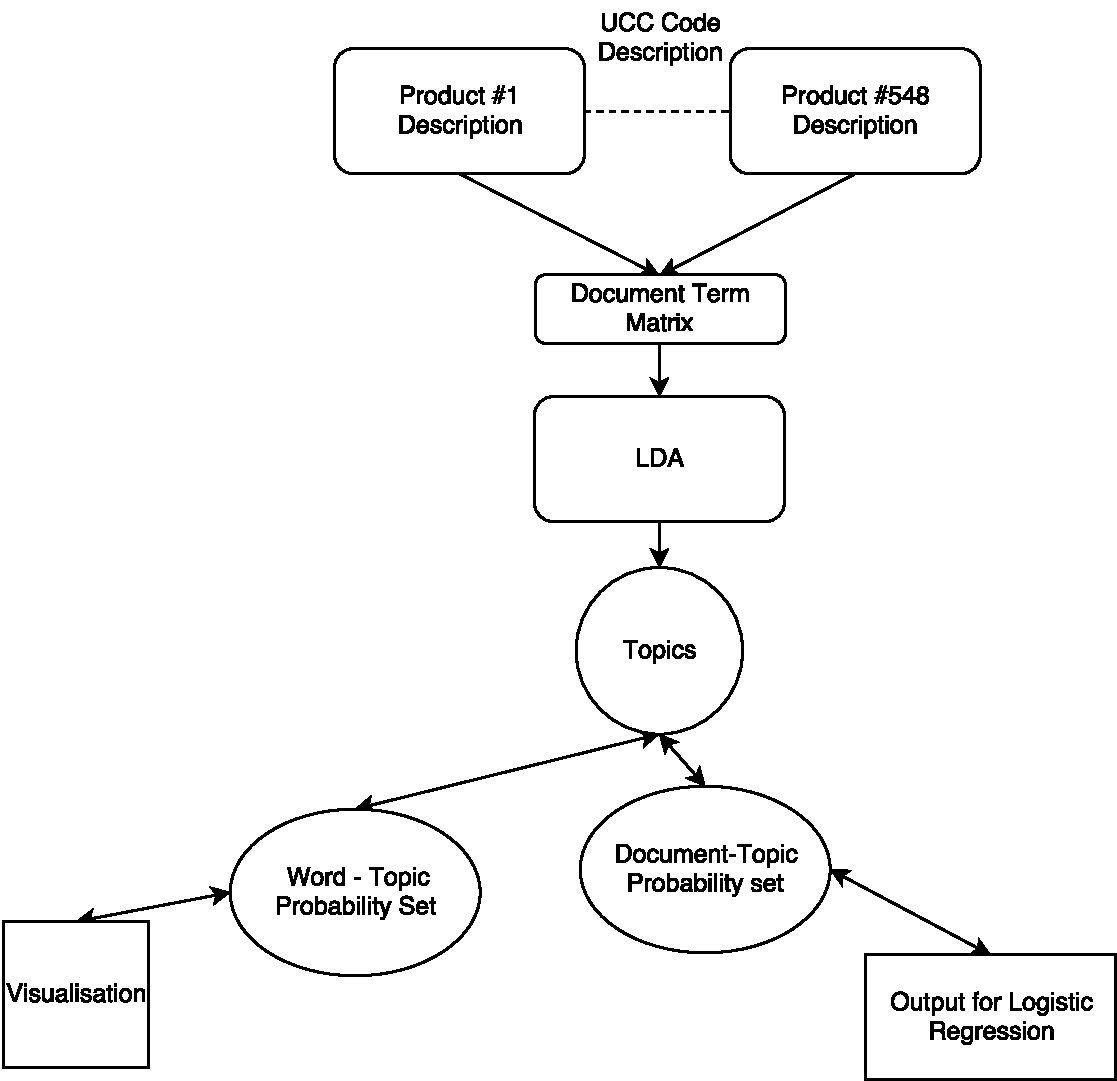
\includegraphics[width=1\textwidth]{/Users/charlvanschoor/Documents/Gottingen/ML/ML-Applications-CVS/LDA_consumer_analysis/paper/content/graphs/LDA.pdf}
\caption{LDA Input-Output Layout}
\end{figure}

\begin{figure}[!h]
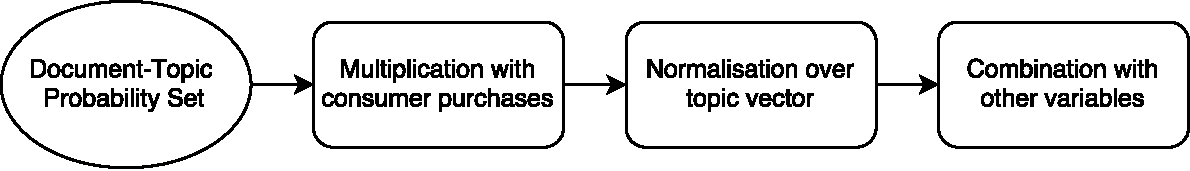
\includegraphics[width=1\textwidth]{/Users/charlvanschoor/Documents/Gottingen/ML/ML-Applications-CVS/LDA_consumer_analysis/paper/content/graphs/norm.pdf}
\caption{Topics to Final Dataset Layout}
\end{figure}

% subsection lda_model (end)

\subsection{Logistic regression} % (fold)
\label{sub:logistic_regression}

The second goal of the paper is to identify which factors explain the most variation in gift purchasing behaviour. To do this I make use of a binomial logistic regression function which uses a logistic distribution log-likelihood function\footnote{The programming software R comes standard with Generalized Linear Models, of which the binomial GLM is used for this paper.}. The purpose of the logistic regression is to act as a baseline for predicting gift purchasing behaviour. The regression structure is as follows:

\

\begin{equation}\centering
GIF{T_i} = \sum\limits_{k = 1}^K {Topi{c_i}(k)}  + AG{E_i} + INCLAS{S_i} + EDUC{A_i} + STATE{_i} + SE{X_i}
\end{equation}
where $i = 1....N$ and $k = 1....L + K$

\

Each variable follows intuitively on the variables specified in the data section of this paper. Notice that the variable "Topic" is a summation over the topic vectors. The reason for this is that various amounts of topics are modeled for the purpose of this paper; the aim of which is to determine what set of topics is optimal for the highest prediction accuracy. The regressions thus models the log-likelihood, or intuitively the probability, that a consumer would purchase a gift or not. The decision boundary is set a 0.5, meaning that a probability below 0.5 is categorized as a 0, whereas a value equal to or above 0.5 is categorized as a 1. 


% subsection logistic_regression (end)

\subsection{Neural Network} % (fold)
\label{sub:neural_network}

The purpose of the neural network is to improve the prediction accuracy of the model, as this method is known to have a higher predictive capability than linear regression models. It has the ability to model non-linear relationships in a black box manner. This is however also the disadvantage of using this technique, as it does not allow for possible causal inference of the variables in the model. 

\

The neural network is set op to train and test the same model as that of the logistic regression model. The total dataset is constructed such that there are the same amount of households that have a value of 1 and 0 for GIFT. In other words, the training and testing datasets have reduced dimensions to account for possible pattern forming. If this is not done, the neural network learns to predict whether a household will not purchase a gift very well, but it falls short of predicting whether a household will purchase a gift. 

\

Moreover, the neural network is constructed with the Keras library that utilizes a TensorFlow backend. The model is set to have one hidden layer with 128 neurons as the nature of the dataset does not require the complexity of more hidden layers. The model includes a 30 percent dropout during training, as this helps the model from overfitting\citep{srivastava2014dropout}. The model also includes cross-validation during the training set to help detect over-fitting and to assist in hyper-parameter optimization. Furthermore, the hidden layer is fitted with a standard sigmoid activation function and the output layer is fitted with 
a softmax activation function\footnote{The decision for which activation function is made on intuition, as both activation functions yields better results.}. The model is fitted with adam as an optimization function, and a binary cross entropy loss function. Th model was set to run a smaller set of epochs with smaller bach sizes in order for it to train at a slower rate. Finally, the metrics used to validate the model is the accuracy of prediction in the test dataset and the optimization of the loss during training. 

% subsection neural_network (end)


% section methodology (end)
  
	\section{Results} % (fold)
\label{sec:results}

 

\subsection{LDA} % (fold)
\label{sub:lda}

The results from the LDA depends on the amount of topics specified. This requires consideration on two parts: First is whether the amount of topics specified makes intuitive sense. The second is what amount of topics produces the highest gift prediction accuracy. Therefore, I created an infrastructure to model a wide set of topics ranging from 2 to 10, and thereafter different intervals ranging from 10 up till a 100 topics\footnote{the source files provided for this paper shows all of the topics modeled as well as figures representing all of the topics. Each of the figures presented in this paper has counterparts for all of the topics in the sources files.}. These  are useful for computing different regression and neural network predictions. However, I stick with 30 topics for the purpose of this section to show how the model performed\footnote{Although there exist test to check the optimal amount of topics within a dataset (such as those developed by \cite{arun2010finding}, \cite{griffiths2004finding} and more) the amount of topics used in this section is based on intuition and is meant to represent the results from the modeling.}. 

\

Figure 3 below represents the product distributions over each of the 30 topics. In other words, the figure shows the total documents likely to be within each topic; each product's, or document's, maximum gamma probability value is taken, thereby allocating it to only a specific topic, thereafter each topic is counted for the amount of products within each topic. The figure shows a good distribution of products over the topics, meaning that the topics do capture a variety of products. This is the aim of using the Wikipedia descriptions of the products, to allocate them into distinct topics without having a single topic, or a set of topics, dominate the entire product space. 


\begin{figure}[!h]
\caption{Product-Topic Distribution}\centering
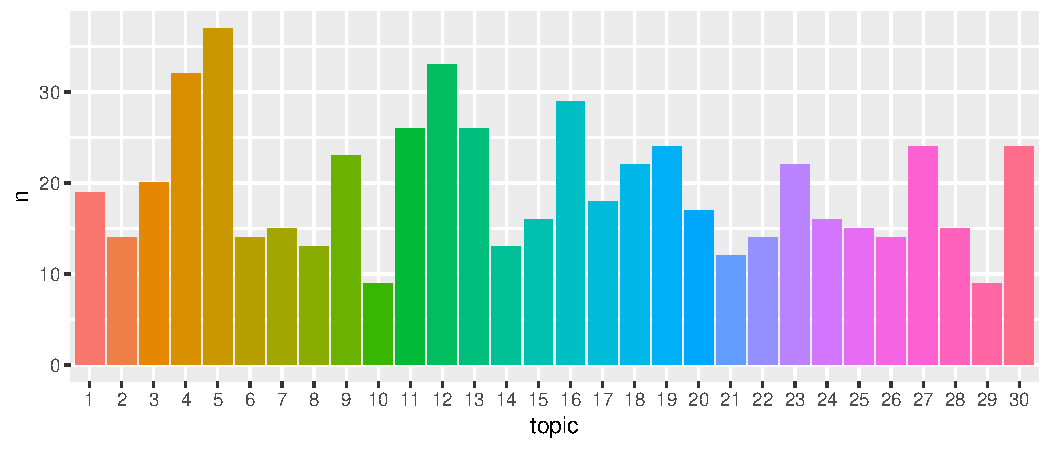
\includegraphics[width=0.9\textwidth]{/Users/charlvanschoor/Documents/Gottingen/ML/ML-Applications-CVS/LDA_consumer_analysis/src/output/product-distribution-per-topic/product-distribution-per-30-topic.pdf}
\end{figure}


\begin{figure}[!h]
\caption{Product-Topic Mixture}\centering
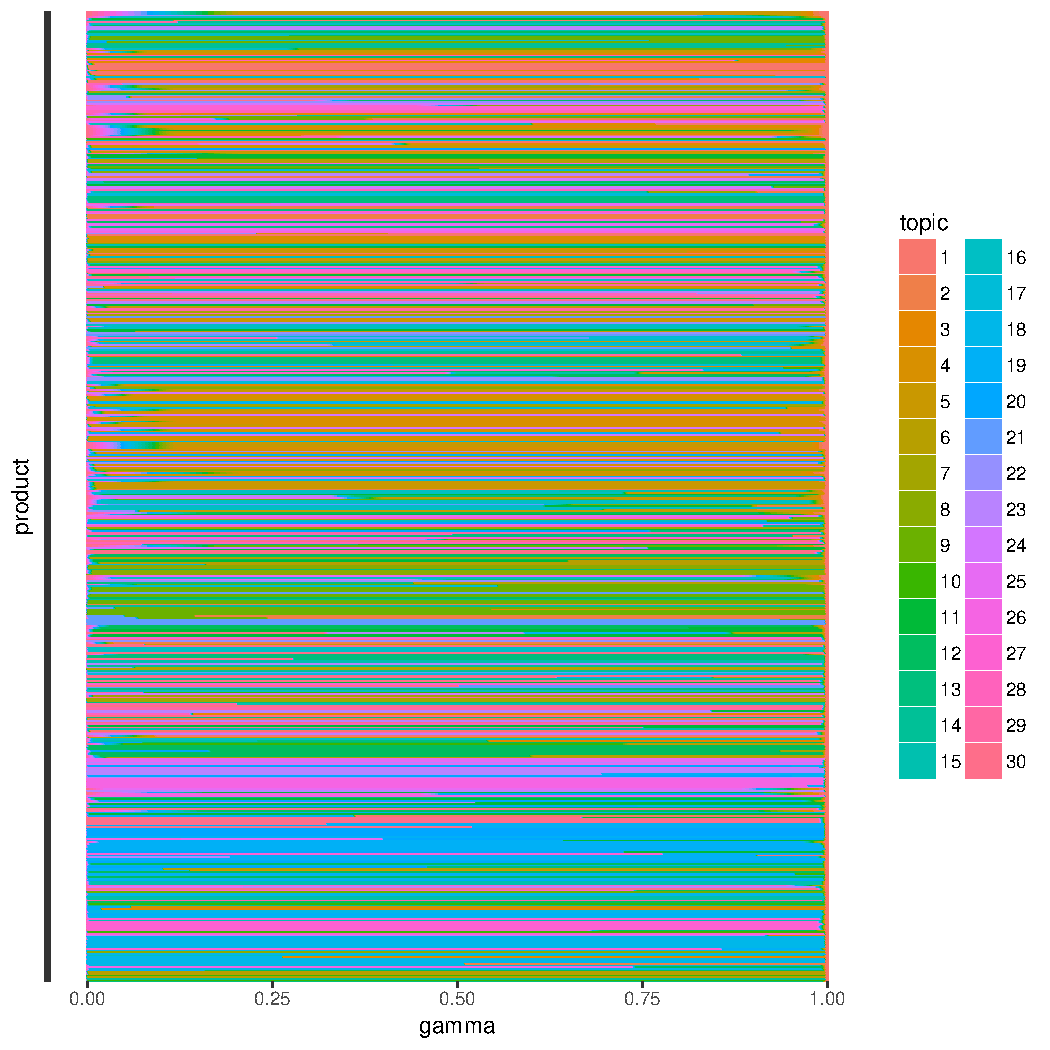
\includegraphics[width=0.9\textwidth]{/Users/charlvanschoor/Documents/Gottingen/ML/ML-Applications-CVS/LDA_consumer_analysis/src/output/topic-distributions-per-product/30-topic-distribution-per-product.pdf}
\end{figure}
\

Moreover, Figure 4 shows a similar story as that of the one above; it shows the gamma probability distributions for each of the products, or documents. In other words, the figure shows the probabilities for each document belonging to each of the 30 topic\footnote{The sources files provided for this paper contains figures representing this for all of the topic sets.}. As visible from the figure, most products are allocated to specific topics; this indicates that most products fall within a certain topic, which is a good result given the origin of the text data. However, some products belong to various topics. Once again, this is not a bad result as it gives some variance to the model. This means that the LDA possibly allocated a probability for complimentary products into the same topics, and probabilities for substitute products into other topics. In other words, some products belong to each other, like vehicles and fuel, and the LDA allocated higher probabilities to those products in the same topic. Some products are substitutes products, like sugar and artificial sweeteners for example, and the LDA possibbly allocated probabilities for those products in the same topic. This means that the LDA might be picking up relationships between the products that are not available when considering the products on their own; it would be tedious for a person to allocate more than 500 products into topics. 


\

\begin{figure}[!h]
\caption{Top 6 Words Over 30 Topics}\centering
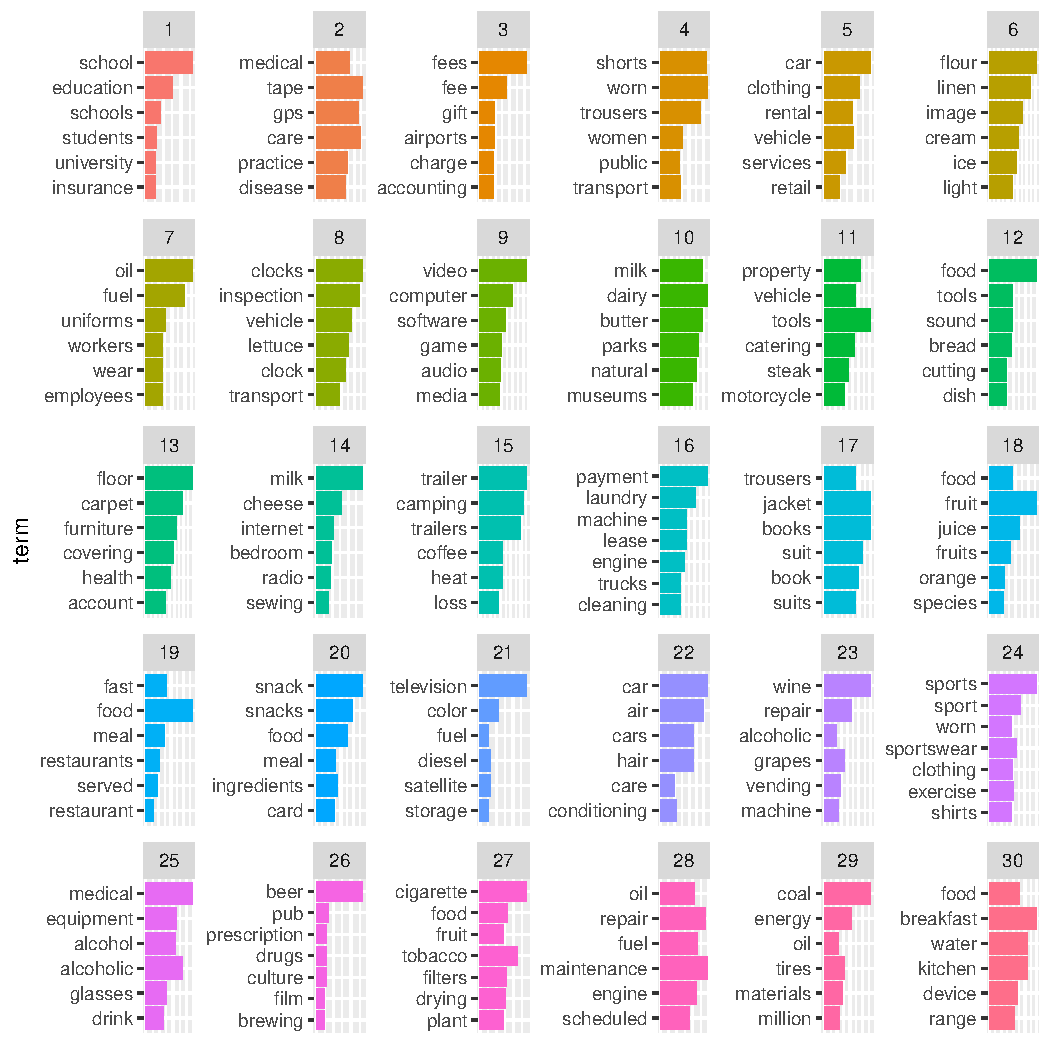
\includegraphics[width=0.9\textwidth]{/Users/charlvanschoor/Documents/Gottingen/ML/ML-Applications-CVS/LDA_consumer_analysis/src/output/top-words-per-topic/top-6-words-in-each30-topics.pdf}
\end{figure}

Figure 5 emphasizes the point made above. The figure shows top 6 words (the maximum beta probabilities for each word) in the 30 topics. There are a few notable topics: Topic 1 represents electronic devices, topic 2 consists of food products, topic 7 represents camping related products and services, topic 12 consists of fast food and restaurant products, topic 23 represents clothing items, topic 29 connects cultural activities etc. The figure shows that the model was able to allocate products that are related to each other. This emphasizes the point that a LDA model requires more information in the documents to allocate products into topics. The result is a mixture of product in each topic that are related in some way, by either cultural or economic principles\footnote{As an economic example, topic 21 relates education with public transport, which makes sense as students use public transport.}. 




% subsection lda (end)


\subsection{Logistic Regression} % (fold)
\label{sub:logistic_regression}


The results from the logistic regression show a compelling story for the inclusion of topics into the model. However, the models seems to show endogeneity, as the significance of the topics far outstretch the significance of the control variables. This is due to the prediction variable used for the model; it is intuitive that the relationship between product and gift purchases is strong, as the one is a direct result of the other. I controlled for this, to some extent, by allocating a binary value to whether a consumer purchased a gift or not, as this eliminates some of the direct relationship between the values. The results do however tell a story, thus we proceed. 

\

Figure 6 shows the top 20 coefficients in terms of significance (sorted by p-value) for the logistic regression that included a 100 topics. The reasoning behind using 100 topics as a representation of the model is due to a few statistics indicating the accuracy and the explanatory power of the model\footnote{The source files provided for this paper contains the results for all of the models with a different set of topics.}. The top 20 predictors are sorted from lowest to the highest p-value. It is clear from the figure that the most significant predictors are the topics\footnote{The source files show that with less topics, around 40, more of the demographic variables are of importance; an intuitive result.}. Topic 73 is the most significant in explaining and predicting gift purchasing behaviour, where topic 99 is the 20th most significant predictor. It is interesting, and intuitive, to note that AGE is the 7th most significant predictor, indicating that generally older households tend to purchase more gifts. The top predictor topics, after inspecting the dataset, contained words such as vehicle, property, truck, agreement, school, bus, students, united, shorts, trousers, sports, electronic etc. Interpreting these results is however difficult, as one does not know exactly what the relationships the topics capture. 

\begin{figure}[!h]
\caption{Top 20 Predictors for 100 Topics}\centering
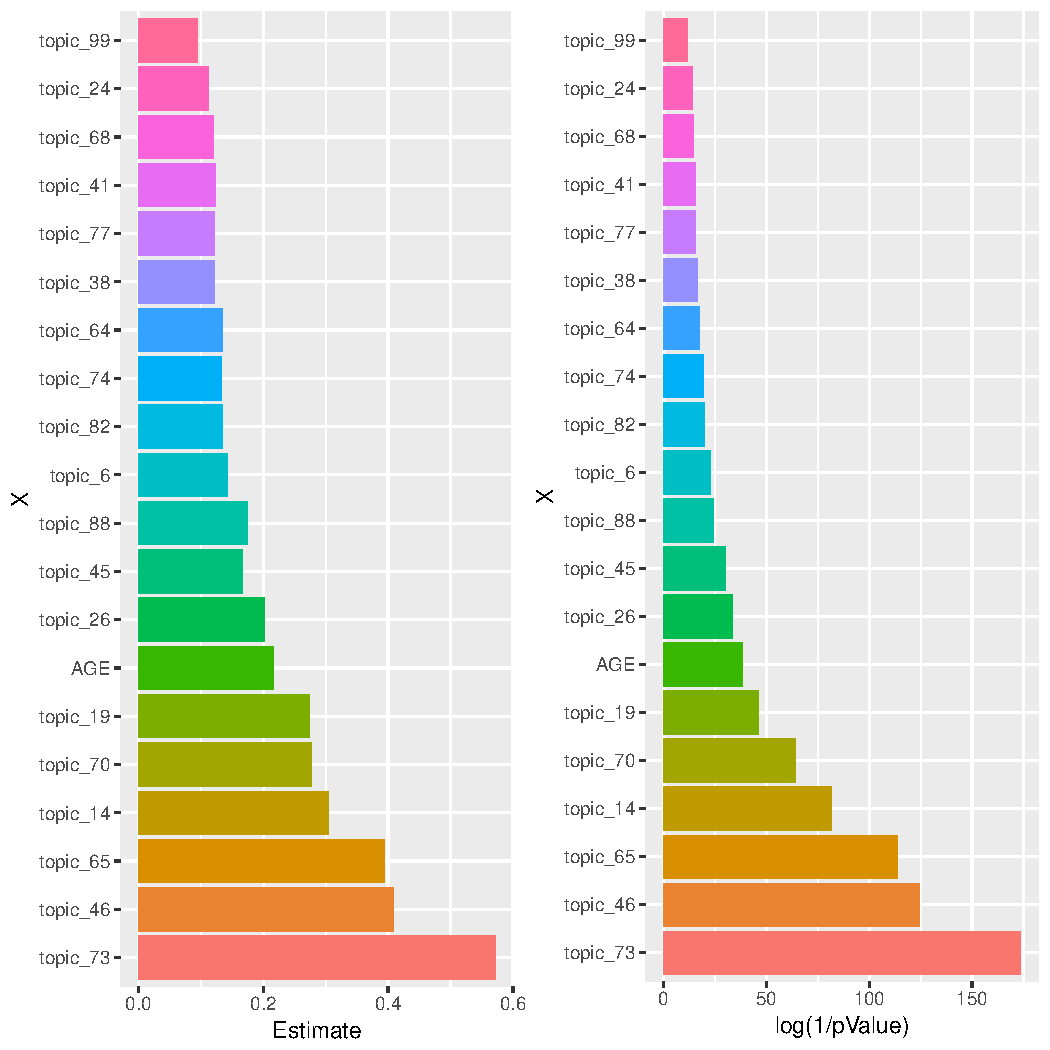
\includegraphics[width=0.7\textwidth]{/Users/charlvanschoor/Documents/Gottingen/ML/ML-Applications-CVS/LDA_consumer_analysis/src/output/GLM-significantPlots/sigPvalue_NUM_TOPICS100.pdf}
\end{figure}

\

It is clear thought that purchases of these types of products are strongly related to gift purchasing behaviour. Note that all of the top predictors are positive, meaning that all increase the likelihood of gift purchasing behaviour. One can speculate that households with property, vehicles, social agreements, children as students etc. have a higher probability of buying gifts. This follows on the intuition of the theoretical background of this paper: Individuals that consider the outcome of their purchases are more probable to exhibit gift giving behaviour. 

\

Figures 7 and 8 show the predictive capability of the logistic regression model. Figure 7 is the confusion matrix from using the 100 topics. As visible from the graph, the model is able to predict non-gift purchasing behaviour well, 86 percent accuracy, but not well with predicting gift purchasing behaviour, 55 percent accuracy. 

\

Moreover, Figure 8 shows various statistics for the model. Some important elements are the Mcfadden R-square value and the balanced accuracy. The Mcfadden R-square value is only 25 percent, meaning that the model as a whole has low explanatory power\footnote{The R-square value for the models with less topics are less than the R-square value for the 100 topic model.}. Moreover, the balanced accuracy, which is a measurement for the predictive power, is 70 percent. In other words, the model only predicts false positives and false negatives 30 percent of the time. Thus, the model does have some predictive capability, but lacks in the prediction of gift purchasing behaviour. 


\begin{figure}[!h]
\caption{Confusion Matrix: Top 20 Predictors for 100 Topics}\centering
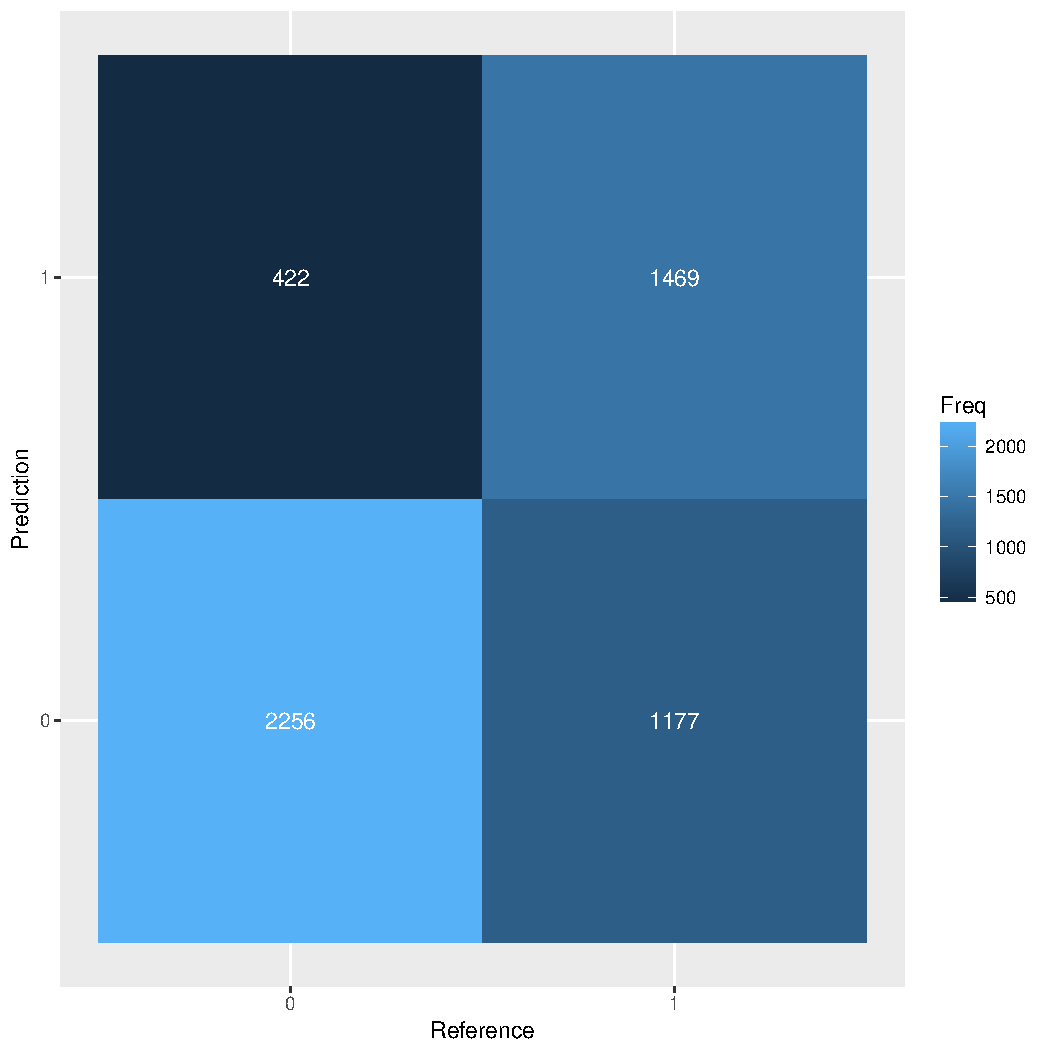
\includegraphics[width=0.5\textwidth]{/Users/charlvanschoor/Documents/Gottingen/ML/ML-Applications-CVS/LDA_consumer_analysis/src/output/confusion-matrices/conf-matrix_NUM_TOPICS100.pdf}
\end{figure}

\begin{figure}[!h]
\caption{Auxiliary Statistics: Top 20 Predictors for 100 Topics}\centering
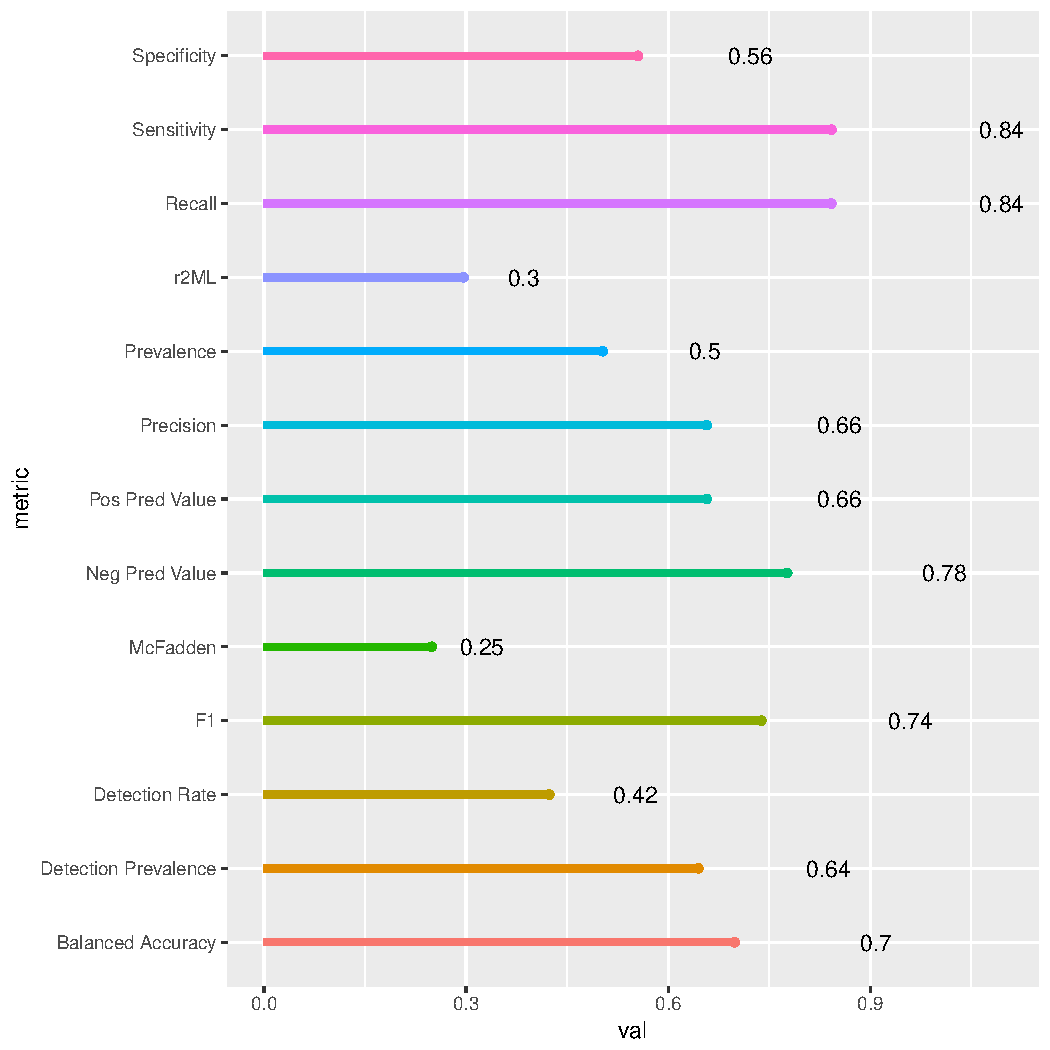
\includegraphics[width=0.8\textwidth]{/Users/charlvanschoor/Documents/Gottingen/ML/ML-Applications-CVS/LDA_consumer_analysis/src/output/confusion-metrics/conf-metrics-_NUM_TOPICS100.pdf}
\end{figure}




% subsection logistic_regression (end)
\subsection{Neural Network} % (fold)
\label{sub:neural_network}

Figures 9 to 12 show the results for the neural network. Each figure reports the results for the models with 10, 50 and a 100 topics. Figure 9 and 10 show the accuracy and loss values for the test dataset. As visible from Figure 9, the neural network has a higher level of accuracy than the logistic regression; around 79 percent for a 100 topics. 

\

Furthermore, the loss function in Figure 10 shows that there is a steady decrease in the loss from the model error, indicating that the model trained well\footnote{The model can be set to learn even slower with smaller batch sizes and more epochs, but this is left for future work.}. Figures 11 and 12 show the validation set accuracy and loss. The errors, or losses in Figure 12, are spread around a mean and can be considered homoscedastic, indicating that the model is not overfitting the data. Thus the neural network improved upon the linear model's predictive power. It is also clear that a model with a 100 topics out-predicts models with a smaller set of topics. This is likely due to the extra information given to the network. It also opens up the question of which amount of topics is optimal, however this is a question for future work.

\begin{figure}[!h]
\caption{Test Accuracy}\centering
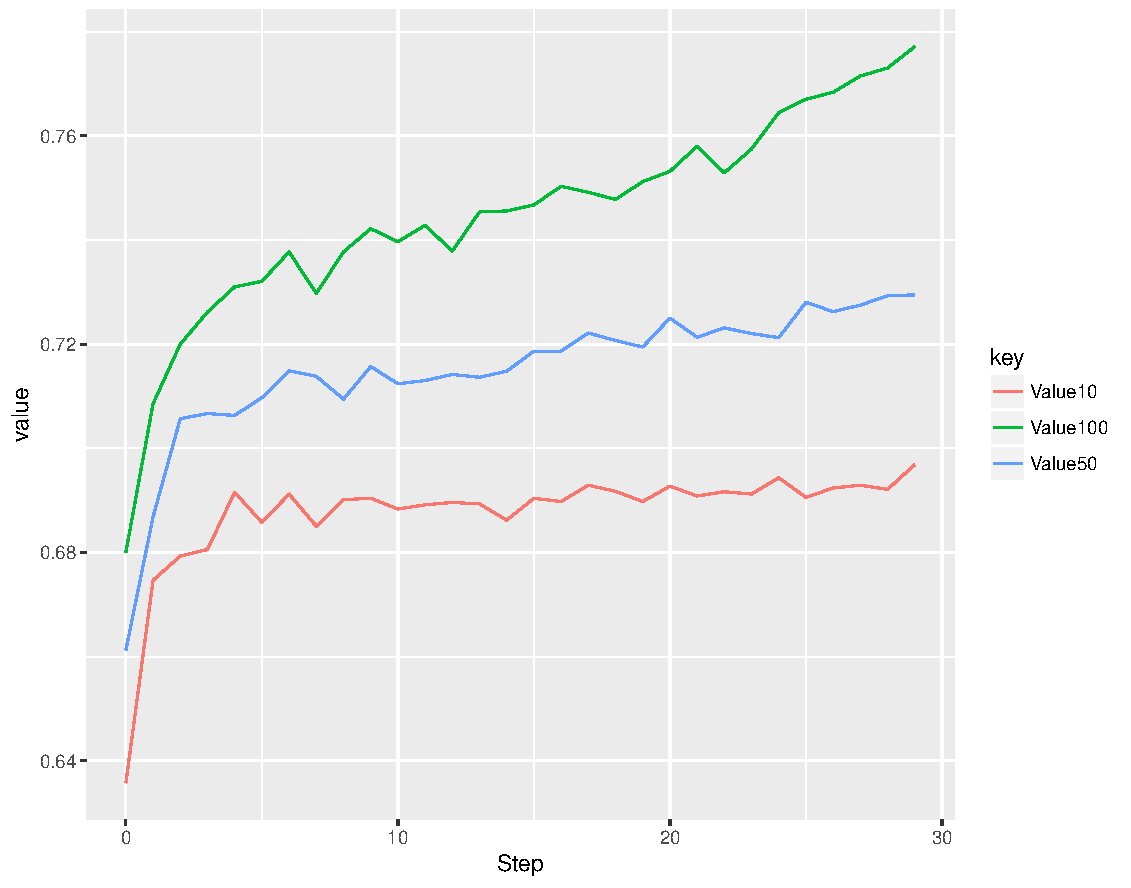
\includegraphics[width=0.7\textwidth]{/Users/charlvanschoor/Documents/Gottingen/ML/ML-Applications-CVS/LDA_consumer_analysis/src/runs/graphs/test_acc.pdf}
\end{figure}


\begin{figure}[!h]
\caption{Test Loss}\centering
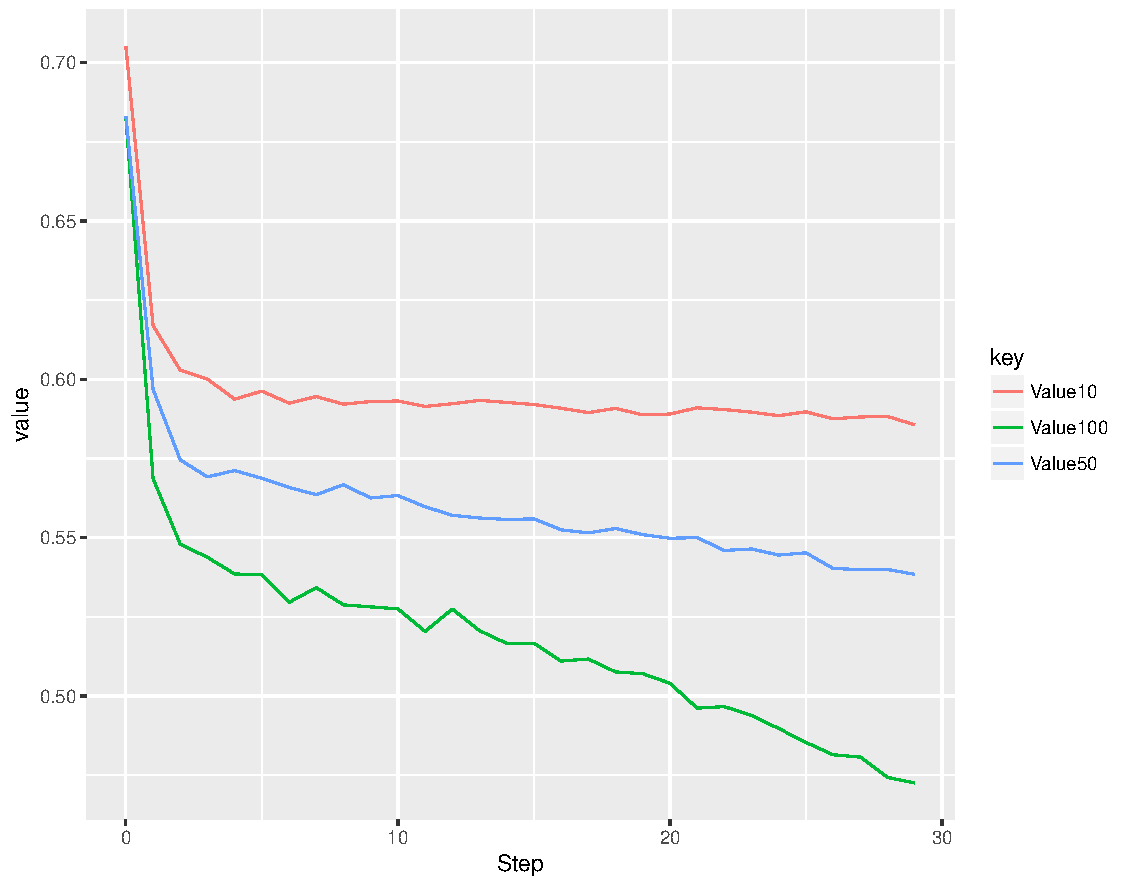
\includegraphics[width=0.7\textwidth]{/Users/charlvanschoor/Documents/Gottingen/ML/ML-Applications-CVS/LDA_consumer_analysis/src/runs/graphs/test_loss.pdf}
\end{figure}


\begin{figure}[!h]
\caption{Validation Accuracy}\centering
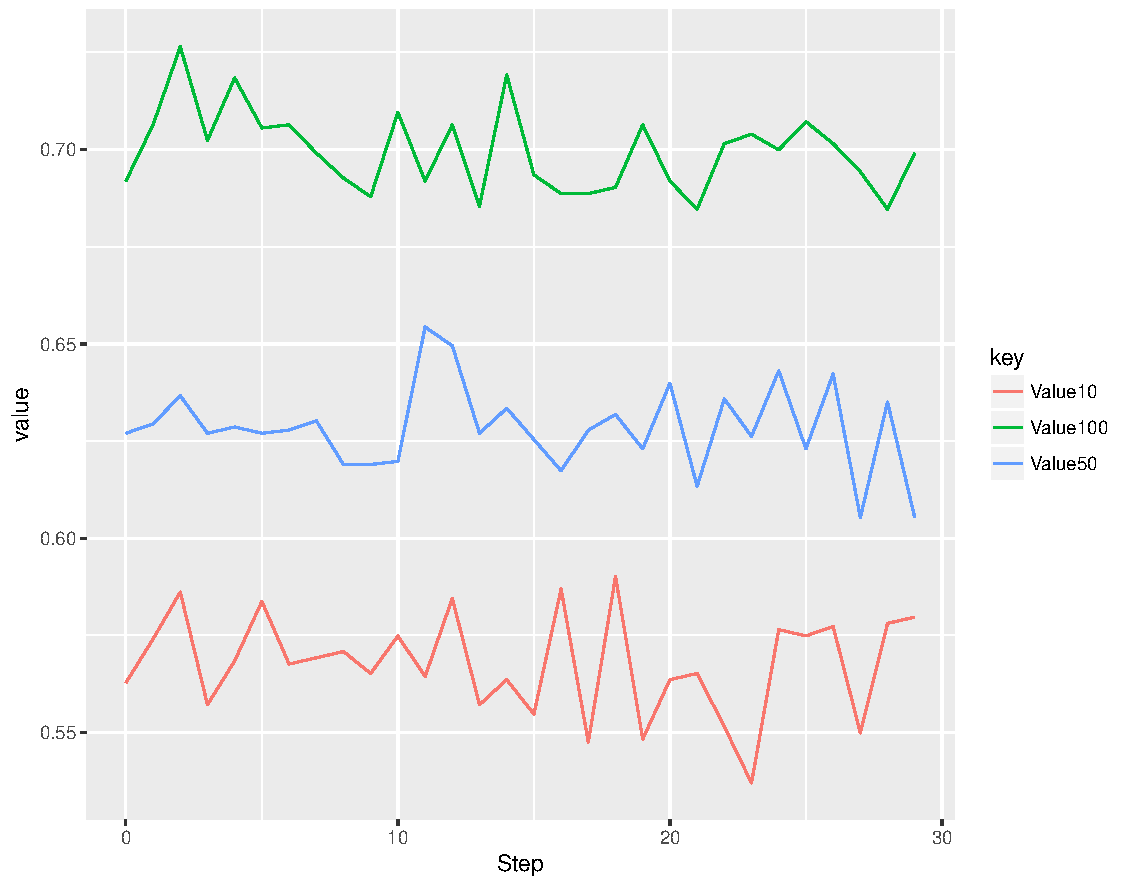
\includegraphics[width=0.7\textwidth]{/Users/charlvanschoor/Documents/Gottingen/ML/ML-Applications-CVS/LDA_consumer_analysis/src/runs/graphs/val_acc.pdf}
\end{figure}


\begin{figure}[!h]
\caption{Validation Loss}\centering
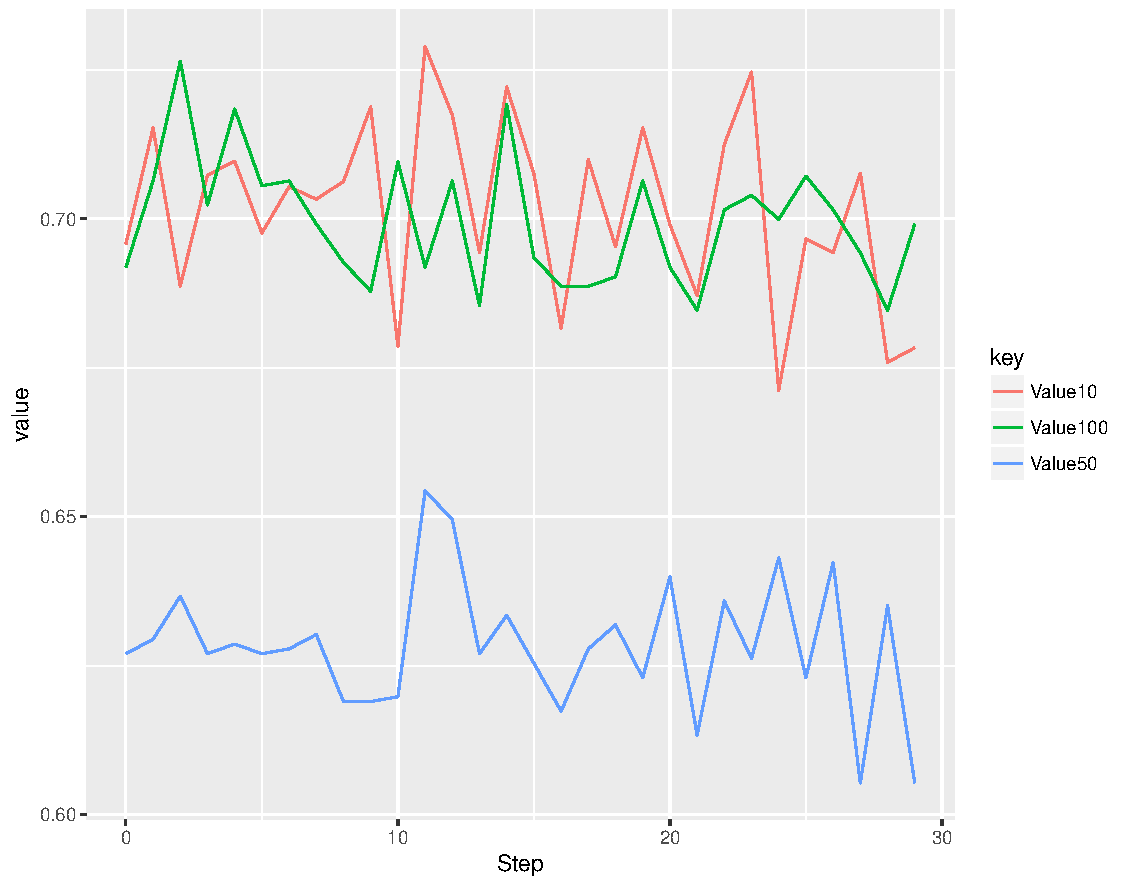
\includegraphics[width=0.7\textwidth]{/Users/charlvanschoor/Documents/Gottingen/ML/ML-Applications-CVS/LDA_consumer_analysis/src/runs/graphs/val_loss.pdf}
\end{figure}

% subsection neural_network (end)

% section results (end)  
	\section{Conclusion} % (fold)
\label{sec:conclusion}


Future work:
find a different, preferably a sequential dataset to have RNN. Use the wiki situation but spend more time removing stop words
specify a different predicted variable to detect whether consumer is utilitarian or hedonic 
Try to use a different measurement to relate consumer purchases with topics 
Use validation processes by having more computational power
Test other models than just NN for prediction 
more research into neural networks for optimal prediction, as the increases in prediction accuracy was not much



% section conclusion (end)
 
	\bibliography{content/bib} \clearpage
	\bibliographystyle{apacite} 
	\section{Appendix} % (fold)
\label{sec:appendix}


\subsection{Tables} % (fold)
\label{sub:tables}

\begin{table}[!h]
\centering
\caption{Variable Descriptions}
\label{my-label}
\begin{adjustbox}{angle=90}
\begin{tabular}{llll}
Full dataset  &                                                                                                                 &                   &           \\
Variable Name & Variable Description                                                                                            & Example           & Dimension \\
NEWID         & NEWID is the variable inditcating each individual houseld survey                                                & 1292531           & 44746*1   \\
UCC           & UCC represents each products unique universal classification code                                               & 10120             & 548*1     \\
Description   & Description describes each individual product                                                                   & Savings acc.      &           \\
N             & The amount of times a product was purchsed by a particular household                                            & 1                 & 1195829*1 \\
Gift          & Gifts represents whether a household purchased a gift or not & 1,0               & 44746*1   \\
AGE           & The average age of a household                                                                                  & 67                & 44746*1   \\
EDUCA         & The maximum level of education within a household                                                               & 8                 & 44746*1   \\
STATE         & The state in which the survey was conducted                                                                     & 51                & 44746*1   \\
SEX           & Whether the household is male or female dominated, or balanced.                                                 & M                 & 44746*1   \\
INCLASS       & The inclome class of the household                                                                              & \textgreater75000 & 44746*1  
\end{tabular}
\end{adjustbox}
\end{table}



% subsection tables (end)
\clearpage



\subsection{Figures} % (fold)
\label{sub:figures}

\begin{figure}[!h]
\caption{Top 10 Words Over 7 Topics}\centering
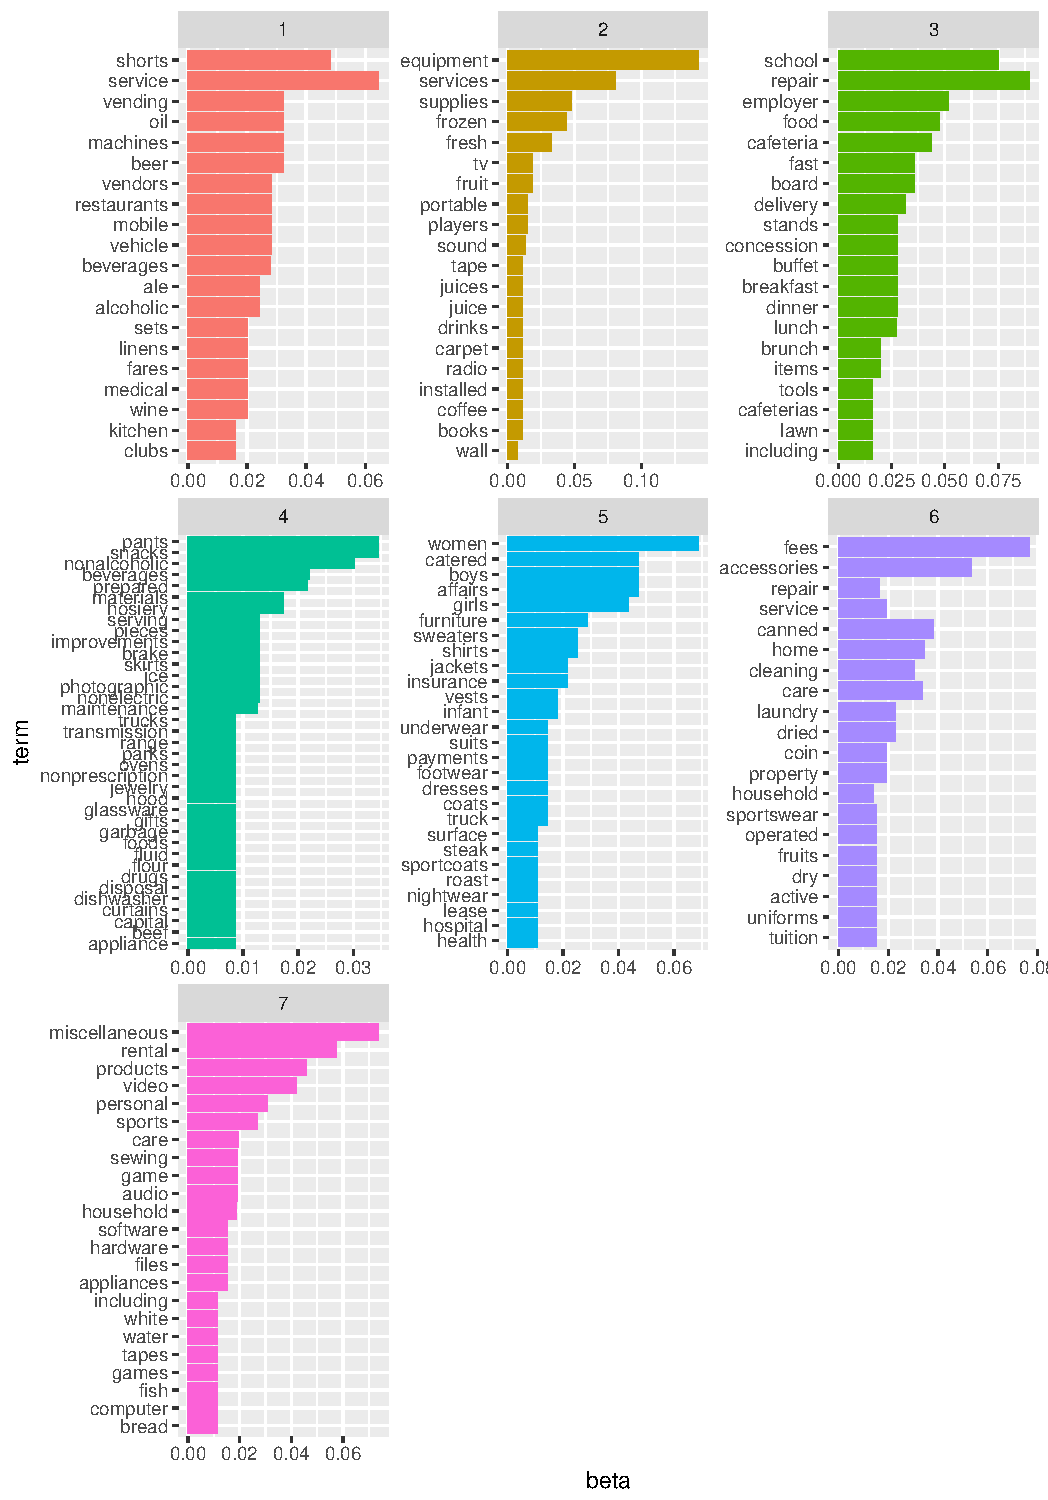
\includegraphics[width=1\textwidth]{/Users/charlvanschoor/Documents/Gottingen/ML/ML-Applications-CVS/LDA_consumer_analysis/paper/content/graphs/topicsper30_before_wiki.pdf}
\end{figure}
\begin{figure}
\caption{Word-Count Per Product}\centering
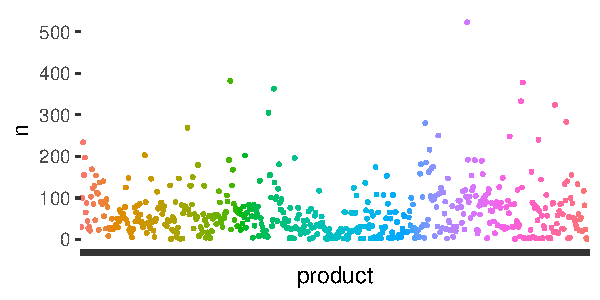
\includegraphics[width=1.1\textwidth]{/Users/charlvanschoor/Documents/Gottingen/ML/ML-Applications-CVS/LDA_consumer_analysis/paper/content/graphs/word-count-per-product.pdf}
\end{figure}

\begin{figure}
\caption{CPP Matrix Visualization}\centering
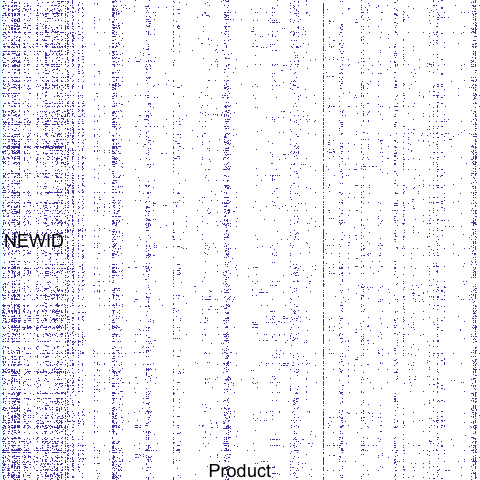
\includegraphics[width=1.1\textwidth]{/Users/charlvanschoor/Documents/Gottingen/ML/ML-Applications-CVS/LDA_consumer_analysis/src/output/CPP-distribution/CPP_distribution.png}
\end{figure}



\begin{figure}
\caption{Distribution of Household Age for Gift and Non-Gift}\centering
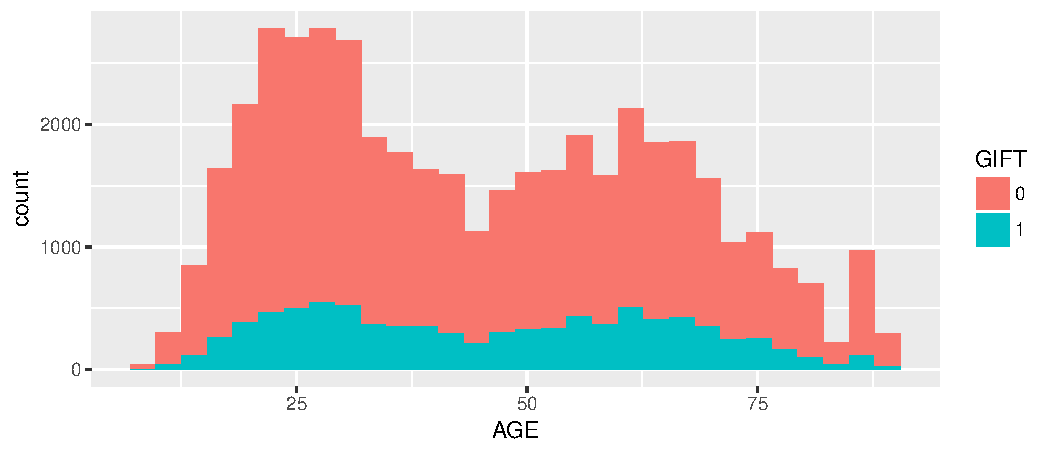
\includegraphics[width=1.1\textwidth]{/Users/charlvanschoor/Documents/Gottingen/ML/ML-Applications-CVS/LDA_consumer_analysis/src/output/CES-distributions/AGE.pdf}
\end{figure}

\begin{figure}
\caption{Distribution of Household Sex for Gift and Non-Gift}\centering
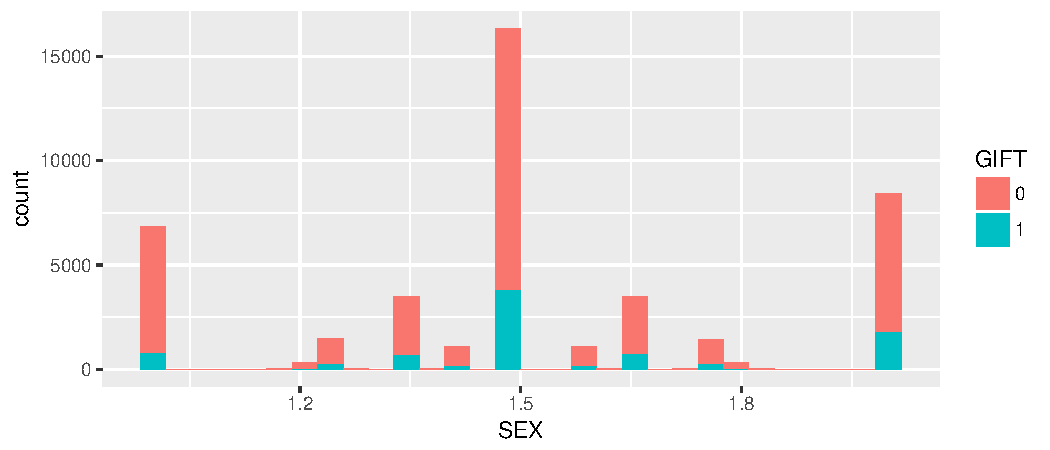
\includegraphics[width=1.1\textwidth]{/Users/charlvanschoor/Documents/Gottingen/ML/ML-Applications-CVS/LDA_consumer_analysis/src/output/CES-distributions/SEX.pdf}
\end{figure}

\begin{figure}
\caption{Distribution of Household Education for Gift and Non-Gift}\centering
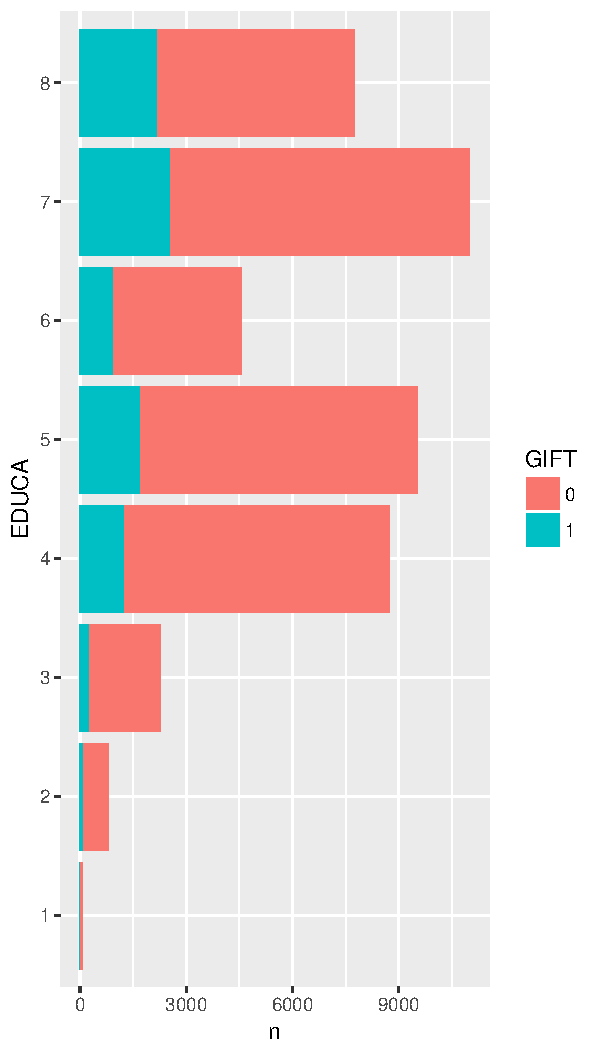
\includegraphics[width=0.8\textwidth]{/Users/charlvanschoor/Documents/Gottingen/ML/ML-Applications-CVS/LDA_consumer_analysis/src/output/CES-distributions/EDUCA.pdf}
\end{figure}

\begin{figure}
\caption{Distribution of Household Income Class for Gift and Non-Gift}\centering
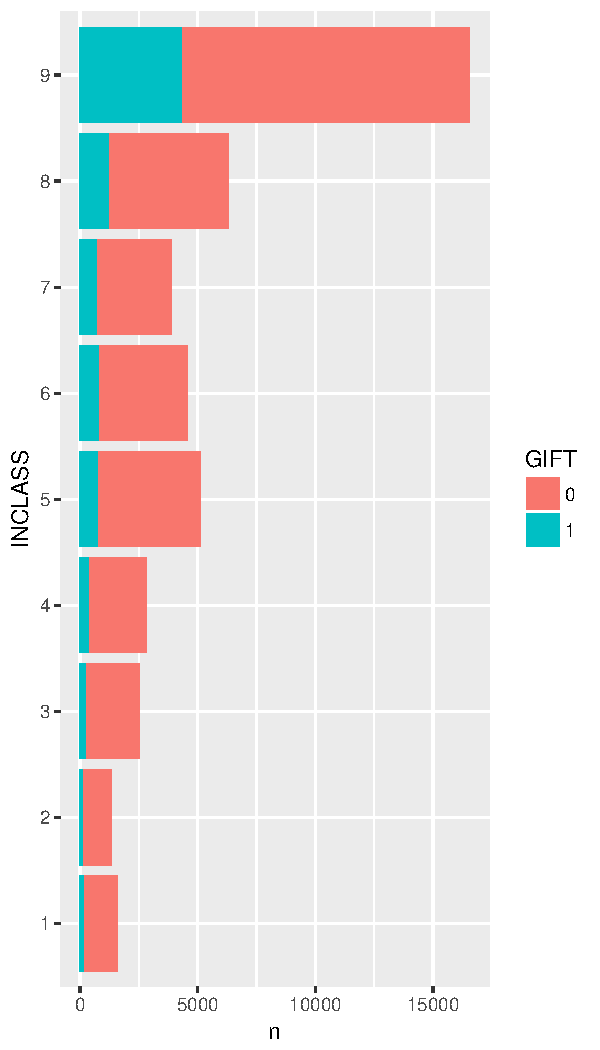
\includegraphics[width=0.8\textwidth]{/Users/charlvanschoor/Documents/Gottingen/ML/ML-Applications-CVS/LDA_consumer_analysis/src/output/CES-distributions/INCLASS.pdf}
\end{figure}



\begin{figure}
\caption{Distribution of State for Gift and Non-Gift}\centering
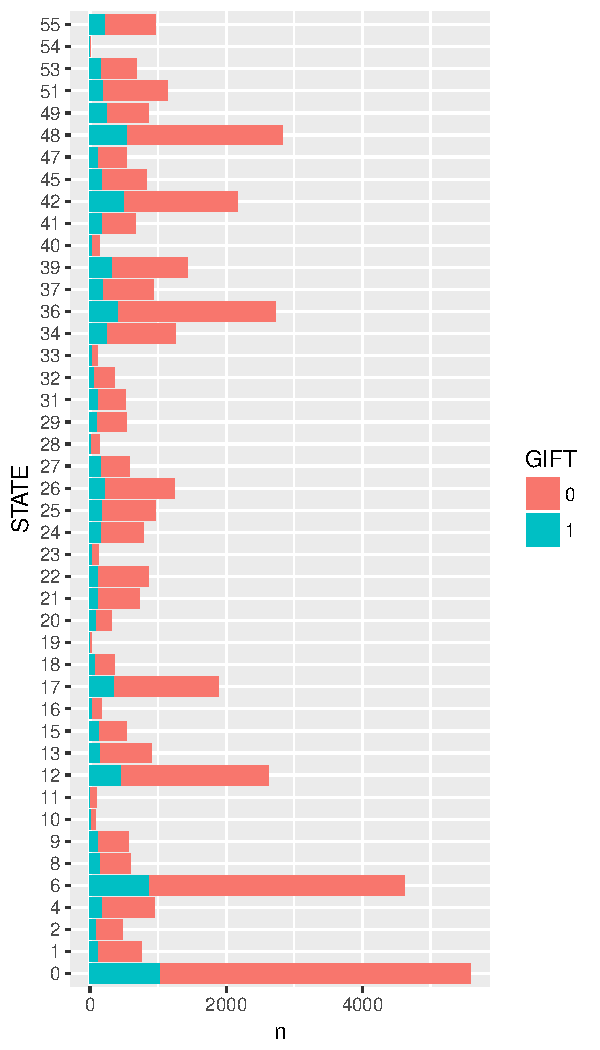
\includegraphics[width=0.8\textwidth]{/Users/charlvanschoor/Documents/Gottingen/ML/ML-Applications-CVS/LDA_consumer_analysis/src/output/CES-distributions/STATE.pdf}
\end{figure}


% subsection figures (end)




% section appendix (end)


	%\section{Appendix} % (fold)
\label{sec:appendix}


\subsection{Tables} % (fold)
\label{sub:tables}

\begin{table}[!h]
\centering
\caption{Variable Descriptions}
\label{my-label}
\begin{adjustbox}{angle=90}
\begin{tabular}{llll}
Full dataset  &                                                                                                                 &                   &           \\
Variable Name & Variable Description                                                                                            & Example           & Dimension \\
NEWID         & NEWID is the variable inditcating each individual houseld survey                                                & 1292531           & 44746*1   \\
UCC           & UCC represents each products unique universal classification code                                               & 10120             & 548*1     \\
Description   & Description describes each individual product                                                                   & Savings acc.      &           \\
N             & The amount of times a product was purchsed by a particular household                                            & 1                 & 1195829*1 \\
Gift          & Gifts represents whether a household purchased a gift or not & 1,0               & 44746*1   \\
AGE           & The average age of a household                                                                                  & 67                & 44746*1   \\
EDUCA         & The maximum level of education within a household                                                               & 8                 & 44746*1   \\
STATE         & The state in which the survey was conducted                                                                     & 51                & 44746*1   \\
SEX           & Whether the household is male or female dominated, or balanced.                                                 & M                 & 44746*1   \\
INCLASS       & The inclome class of the household                                                                              & \textgreater75000 & 44746*1  
\end{tabular}
\end{adjustbox}
\end{table}



% subsection tables (end)
\clearpage



\subsection{Figures} % (fold)
\label{sub:figures}

\begin{figure}[!h]
\caption{Top 10 Words Over 7 Topics}\centering
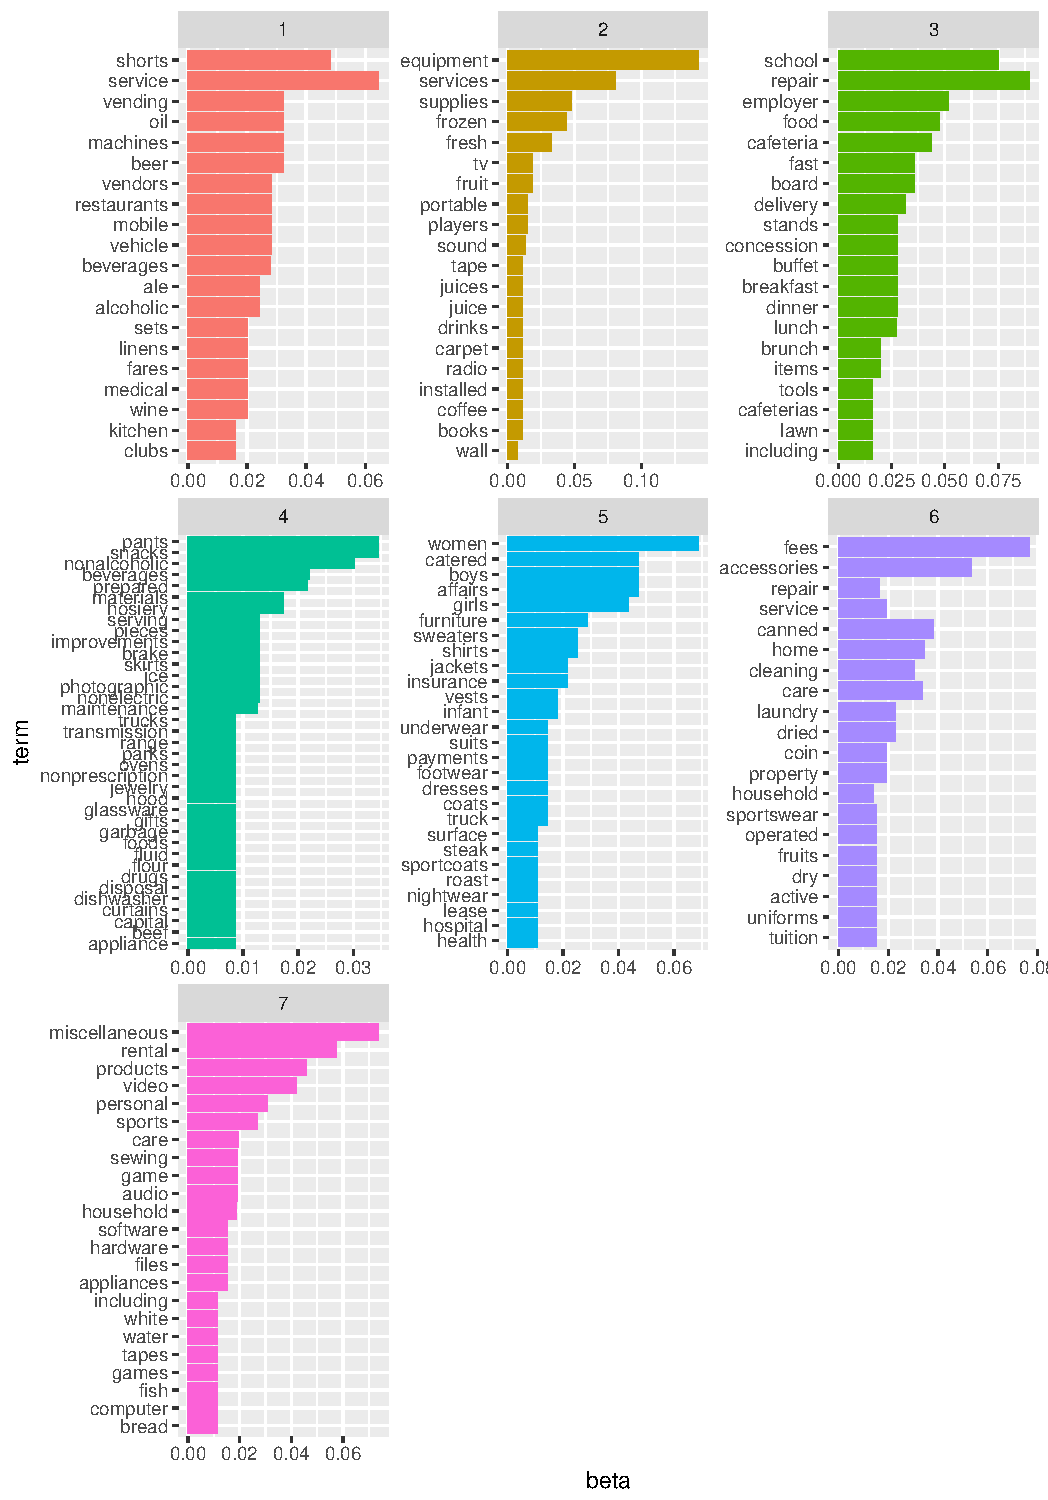
\includegraphics[width=1\textwidth]{/Users/charlvanschoor/Documents/Gottingen/ML/ML-Applications-CVS/LDA_consumer_analysis/paper/content/graphs/topicsper30_before_wiki.pdf}
\end{figure}
\begin{figure}
\caption{Word-Count Per Product}\centering
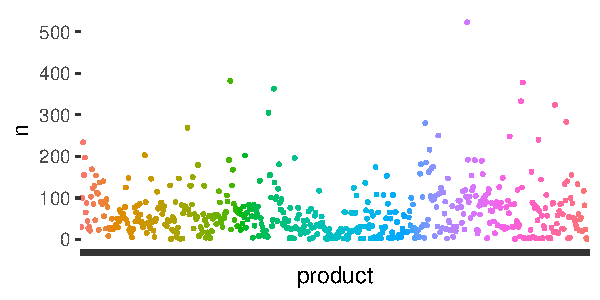
\includegraphics[width=1.1\textwidth]{/Users/charlvanschoor/Documents/Gottingen/ML/ML-Applications-CVS/LDA_consumer_analysis/paper/content/graphs/word-count-per-product.pdf}
\end{figure}

\begin{figure}
\caption{CPP Matrix Visualization}\centering
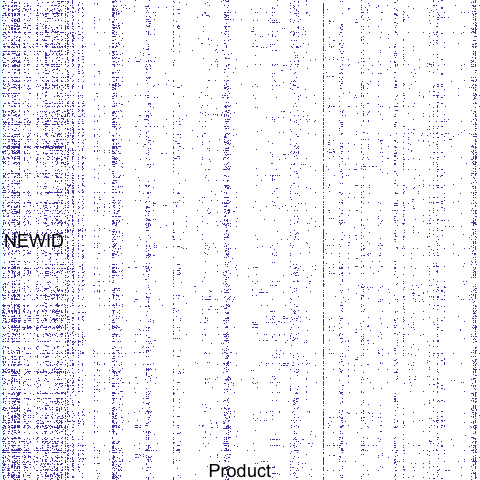
\includegraphics[width=1.1\textwidth]{/Users/charlvanschoor/Documents/Gottingen/ML/ML-Applications-CVS/LDA_consumer_analysis/src/output/CPP-distribution/CPP_distribution.png}
\end{figure}



\begin{figure}
\caption{Distribution of Household Age for Gift and Non-Gift}\centering
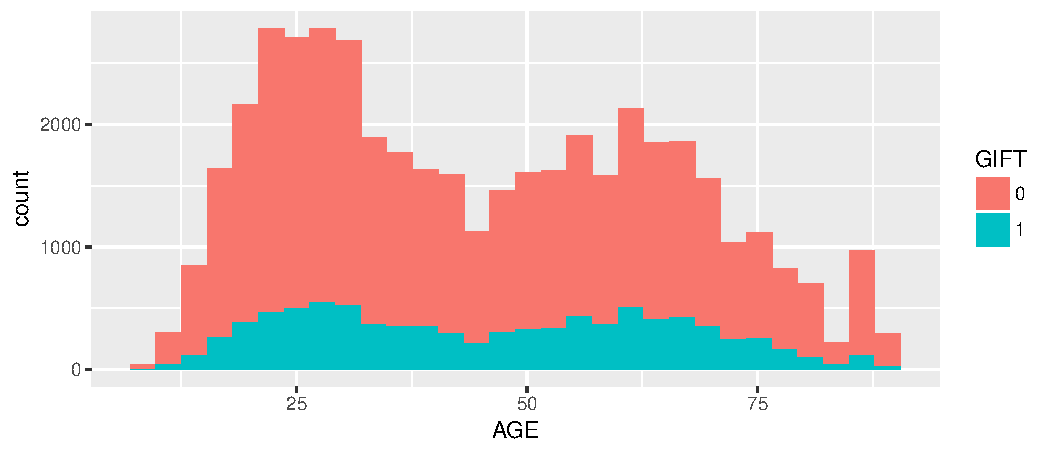
\includegraphics[width=1.1\textwidth]{/Users/charlvanschoor/Documents/Gottingen/ML/ML-Applications-CVS/LDA_consumer_analysis/src/output/CES-distributions/AGE.pdf}
\end{figure}

\begin{figure}
\caption{Distribution of Household Sex for Gift and Non-Gift}\centering
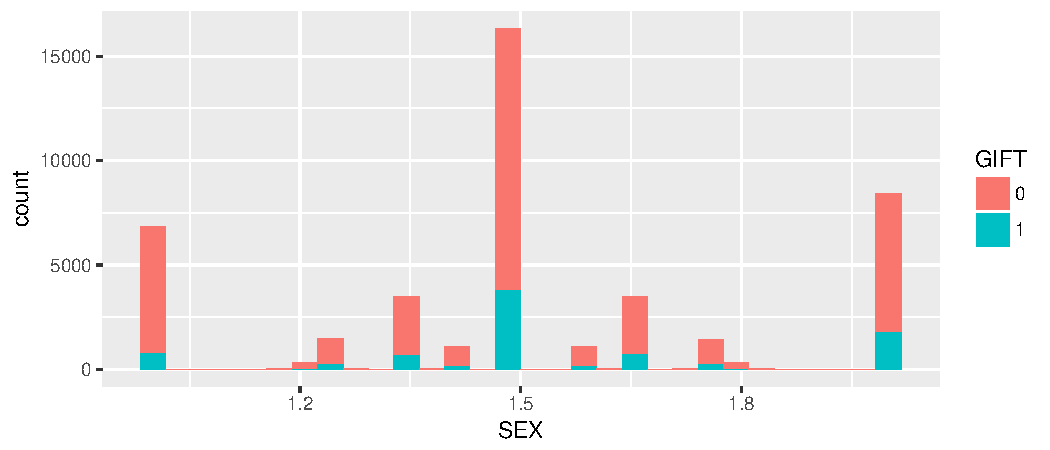
\includegraphics[width=1.1\textwidth]{/Users/charlvanschoor/Documents/Gottingen/ML/ML-Applications-CVS/LDA_consumer_analysis/src/output/CES-distributions/SEX.pdf}
\end{figure}

\begin{figure}
\caption{Distribution of Household Education for Gift and Non-Gift}\centering
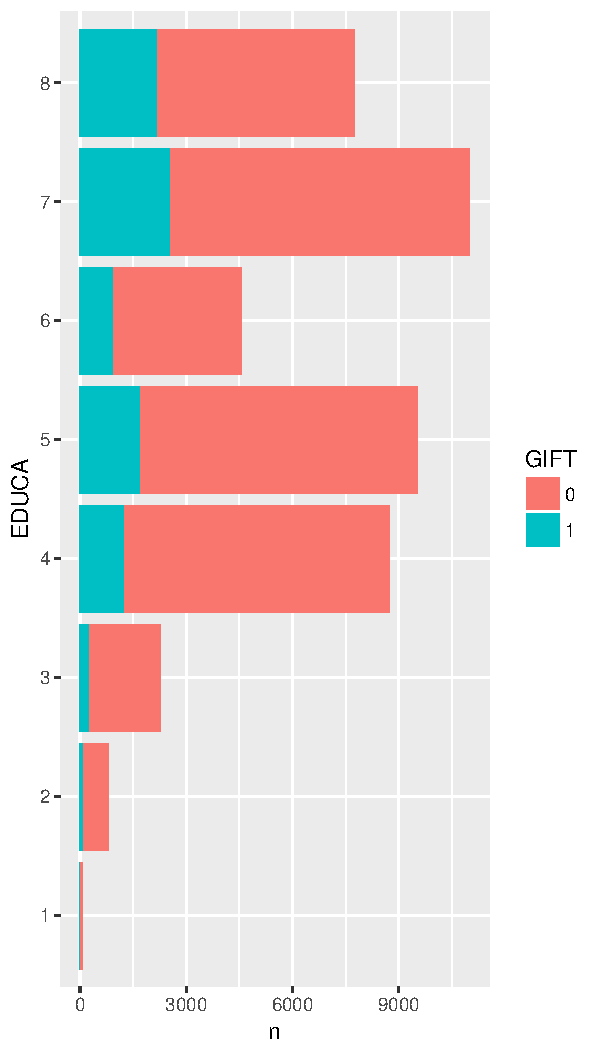
\includegraphics[width=0.8\textwidth]{/Users/charlvanschoor/Documents/Gottingen/ML/ML-Applications-CVS/LDA_consumer_analysis/src/output/CES-distributions/EDUCA.pdf}
\end{figure}

\begin{figure}
\caption{Distribution of Household Income Class for Gift and Non-Gift}\centering
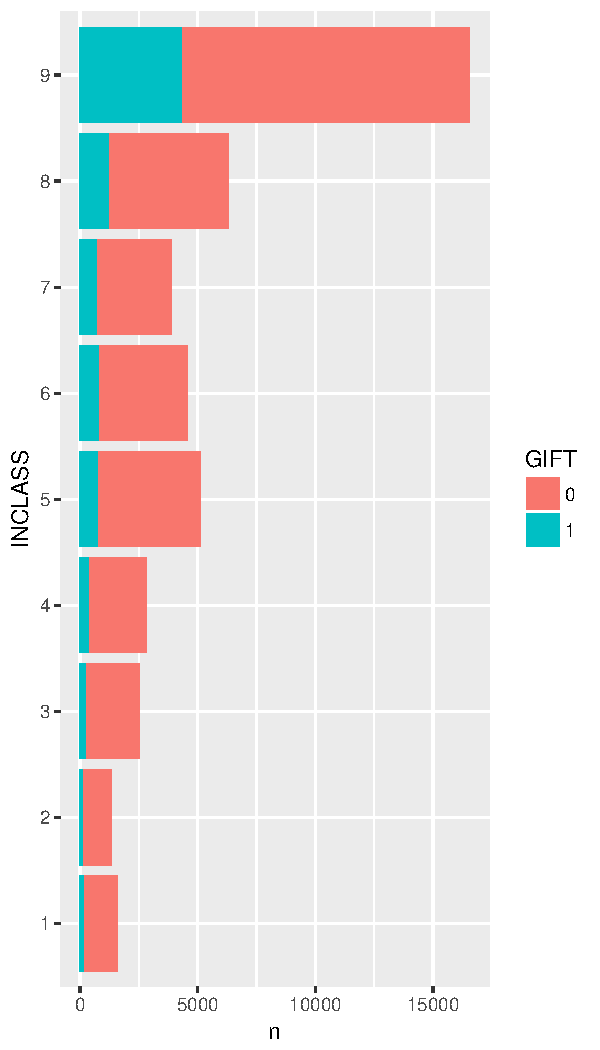
\includegraphics[width=0.8\textwidth]{/Users/charlvanschoor/Documents/Gottingen/ML/ML-Applications-CVS/LDA_consumer_analysis/src/output/CES-distributions/INCLASS.pdf}
\end{figure}



\begin{figure}
\caption{Distribution of State for Gift and Non-Gift}\centering
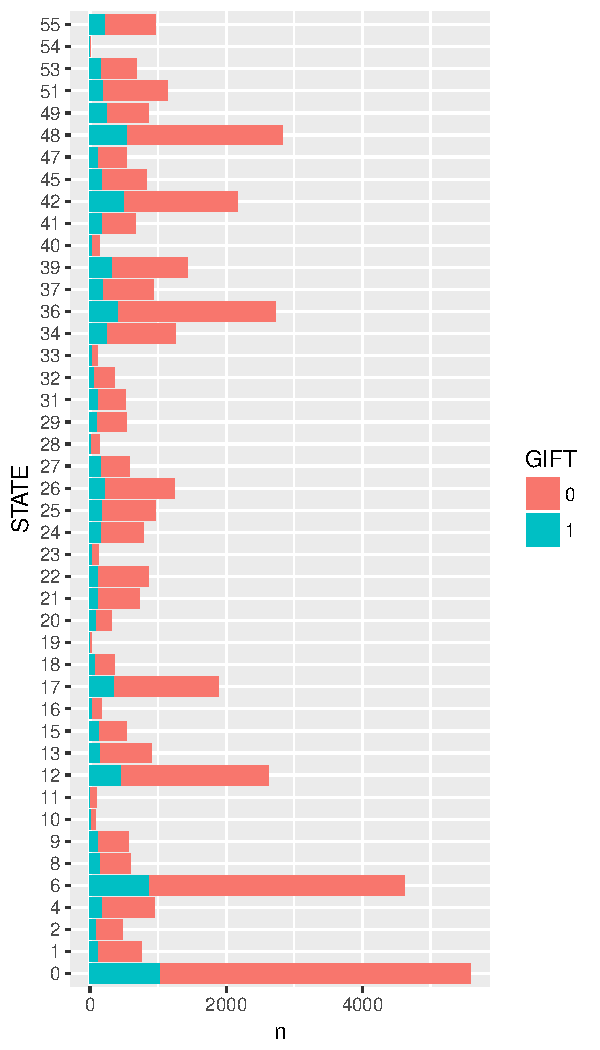
\includegraphics[width=0.8\textwidth]{/Users/charlvanschoor/Documents/Gottingen/ML/ML-Applications-CVS/LDA_consumer_analysis/src/output/CES-distributions/STATE.pdf}
\end{figure}


% subsection figures (end)




% section appendix (end) 
 
	


	





\end{document}
